\documentclass[a4paper,10pt]{article}
\usepackage[utf8]{inputenc}
\usepackage{amsmath}
\usepackage{amssymb}
\usepackage{amsfonts}

\usepackage{color}
\definecolor{linkcol}{rgb}{0,0,0.4}
\definecolor{citecol}{rgb}{0.5,0,0}

\usepackage[pagebackref,hyperindex=true]{hyperref}
\hypersetup{colorlinks=true,linkcolor=linkcol,citecolor=citecol,urlcolor=linkcol}

\usepackage{amsmath}
\usepackage{amssymb}
\usepackage{amsfonts}
\usepackage{amsopn}
\usepackage{braket}
\usepackage{bbm}
\usepackage{dsfont}
\usepackage{kpfonts}
% \usepackage{mathabx}

\parindent=0cm


% Various new commands that ease typesetting math even further
% \newcommand{\assign}{\ensuremath{\coloneq}}
% \newcommand{\rassign}{\ensuremath{\eqcolon}}
\newcommand{\assign}{\ensuremath{:=}}
\newcommand{\rassign}{\ensuremath{=:}}

\newcommand{\of}[1]{\ensuremath{\left( #1 \right)}}
\newcommand{\ofs}[1]{\ensuremath{\left( #1 \right)}}

\newcommand{\norm}[1]{\ensuremath{\| #1 \|}}

\newcommand{\tmop}[1]{\ensuremath{\operatorname{#1}}}

\newcommand{\id}{\ensuremath{\mathds{1}}}
% \newcommand{\id}{\ensuremath{I}}


\newcommand{\conj}[1]{\ensuremath{\overline{#1}}}

\newcommand{\T}{\ensuremath{{}^{\textnormal{T}}}}
\newcommand{\herm}{\ensuremath{{}^{\textnormal{H}}}}

\newcommand{\ft}[1]{\ensuremath{\mathcal{F}\left(#1\right)}}
\newcommand{\ift}[1]{\ensuremath{\mathcal{F}^{-1}\left(#1\right)}}

\newcommand{\fft}[1]{\ensuremath{\mathtt{FFT}\left(#1\right)}}
\newcommand{\ifft}[1]{\ensuremath{\mathtt{IFFT}\left(#1\right)}}

\newcommand{\dotp}[2]{\ensuremath{\langle #1 , #2 \rangle}}

\newcommand{\bigO}[1]{\ensuremath{\mathcal{O}\left( #1 \right)}}

\newcommand{\mat}[1]{\ensuremath{\mathbf{#1}}}

% multi-indices
\newcommand{\mindex}[1]{\ensuremath{\underline{#1}}}

\newcommand{\laplace}{\ensuremath{\operatorname{\Delta}}}

% EOF

\usepackage{graphicx}
\usepackage{subcaption}
\usepackage{asymptote}
\usepackage{tikz}
\usetikzlibrary{shapes,arrows}


\synctex=1

%opening
\title{Numerical Steepest Descent for Wavepackets II}
\author{R. Bourquin}

\parindent 0pt

\begin{document}

\maketitle


\section{Primary task}

Given functions $f(x_1, \ldots, x_n):\mathbb{R^N}\rightarrow\mathbb{R}$ and
$g(x_1, \ldots, x_n):\mathbb{R^N}\rightarrow\mathbb{C}$, compute the integral:

\begin{equation} \label{eq:hoi}
 I := \int_{-\infty}^{\infty} \cdots \int_{-\infty}^{\infty} f \exp(i \omega g) \, \mathrm{d}x_1 \cdots \mathrm{d}x_n
\end{equation}

This is a highly oscillatory integral. Usually we call $g$ the \emph{oscillator}
and $f$ the \emph{amplitude} or \emph{enveloppe}. For more details see the work
by Huybrechs and some others. The main technique is described in \cite{HV_hoq} for
the one-dimensional case and in \cite{HV_cub} for multivariate integrands.
Semi-infinite intervalls are treated in \cite{H_nsd_sii}.


\section{One-dimensional examples}

We want to compute the following integral:

\begin{equation} \label{eq:oscillatory_integral}
 I := \int_{-\infty}^{\infty} f(x) \exp(i \omega g(x)) \mathrm{d}x
\end{equation}

with $f$ reasonable and $g$ quadratic.


\subsection{Oscillator without linear term}
\label{sec:scal_nlt}

Assume we have:

\begin{equation}
 g(x) := a x^2 + c
\end{equation}

Then for the derivatives of $g$ we have:

\begin{equation}
 g^\prime = \pdiff{g}{x} = 2 a x
\end{equation}

and from that solve $g^\prime(x^{*}) = 0$ to find the stationary point $x^{*} = 0$.

The path equation for the integration path becomes:

\begin{equation}
\begin{split}
  g\left( h(t) \right) & = g(x^{*}) + i t \\
  g\left( h(t) \right) & = g(0) + i t \\
  a h^2(t) + c         & = c +  it
\end{split}
\end{equation}

from which we get:

\begin{equation}
 h(t) := \pm \sqrt{\frac{i t}{a}} \,.
\end{equation}

Note that the constant term drops off.
The derivative of the integration path is:

\begin{equation}
 h^{\prime}(t) = \pdiff{h}{t} = \pm \frac{\sqrt{i}}{2\sqrt{a}\sqrt{t}} \,.
\end{equation}

By the variable transformation $x \rightarrow h(t)$ we write the above
integral as:

\begin{equation}
\begin{split}
 I & := \int_{-\infty}^{\infty} f(x) \exp(i \omega g(x)) \mathrm{d}x \\
   &  = \int_{0}^{\infty} f\left(h(t)\right) \exp(i \omega g\left(h(t)\right)) \pdiff{h(t)}{t} \mathrm{d}t \\
   &  = \int_{0}^{\infty} f\left(h(t)\right) \exp\left(i \omega \left(a\frac{i t}{a}+c\right)\right) \pdiff{h(t)}{t} \mathrm{d}t \\
   &  = \exp\left(i \omega c\right)
        \int_{0}^{\infty} f\left(h(t)\right) \exp\left(-\omega t\right) \pdiff{h(t)}{t} \mathrm{d}t
\end{split}
\end{equation}

This integral is solved trivially by generalized Gauss-Laguerre quadrature.


\subsection{Oscillator with linear term}
\label{sec:scal_full}

This time consider:

\begin{equation}
 g(x) := a x^2 + b x + c
\end{equation}

The derivative of $g$ becomes:

\begin{equation}
 g^\prime = \pdiff{g}{x} = 2 a x + b
\end{equation}

and from that we find the stationary point to be $x^{*} = -\frac{b}{2a}$. We
transform $g$ to get rid of the linear term by completing the square:

\begin{equation}
\begin{split}
 g(x) & = \left(\sqrt{a} x + \frac{b}{2\sqrt{a}}\right)^2 - \frac{b^2}{4a} + c \\
      & = a \left(x + \frac{b}{2a}\right)^2 \underbrace{- \frac{b^2}{4a} + c}_{\mathcal{C}} \\
\end{split}
\end{equation}

Defining a new variable $\tilde{x}$ by applying the transformation $\chi$:

\begin{equation}
 \tilde{x} = \chi^{-1}(x) := x + \frac{b}{2a} \quad \leftrightarrow \quad x = \chi(\tilde{x}) = \tilde{x} - \frac{b}{2a}
\end{equation}

and noting that $\mathcal{C} = g\left(x^{*}\right)$ constant we
can write $\tilde{g}$ like:

\begin{equation}
 \tilde{g}\left(\tilde{x}\right) = a \tilde{x}^2 + g\left(x^{*}\right)
\end{equation}

with stationary point $\tilde{x}^{*} = 0$. With this $\tilde{g}$ we are back
in the case from above. We can set up the path equation for a path $\tilde{h}(t)$:

\begin{equation}
\begin{split}
 \tilde{g}\left(\tilde{h}(t)\right) & = \tilde{g}\left(\tilde{x}^{*}\right) + it \\
 \tilde{g}\left(\tilde{h}(t)\right) & = \tilde{g}\left(0\right) + it \\
 a \tilde{h}^2(t) + g\left(x^{*}\right) & = g\left(x^{*}\right) + it
\end{split}
\end{equation}

from where we find:

\begin{equation}
 \tilde{h}(t) := \pm \sqrt{\frac{i t}{a}}
 \quad \mathrm{and} \quad
 \tilde{h}^{\prime}(t) = \pdiff{\tilde{h}}{t} = \pm \frac{\sqrt{i}}{2\sqrt{a}\sqrt{t}} \,.
\end{equation}

Now it is time to apply the back transformation $\chi$ and find:

\begin{equation}
 h(t) = \chi \left(\tilde{h}(t)\right) = \tilde{h}(t) - \frac{b}{2a} \,.
\end{equation}

% for the derivative we have:
%
% \begin{equation}
%  h^\prime(t) = \pdiff{h}{t} = \pdiff{\chi}{\tilde{h}} \pdiff{\tilde{h}}{t}
% \end{equation}
%
% but since $\pdiff{\chi}{\tilde{h}} = 1$ this simply is:
%
% \begin{equation}
%  h^\prime(t) = \pdiff{\tilde{h}}{t} \,.
% \end{equation}

After that we are ready to rewrite the integral again as:

% \begin{equation}
% \begin{split}
%  I & := \int_{-\infty}^{\infty} f(x) \exp(i \omega g(x)) \mathrm{d}x \\
%    &  = \int_{-\infty}^{\infty} f\left(\chi\left(\tilde{x}\right)\right)
%                                 \exp\left(i \omega g\left(\chi\left(\tilde{x}\right)\right)\right) \mathrm{d}\tilde{x} \\
%    &  = \exp\left(i \omega g\left(x^{*}\right)\right)
%         \int_{0}^{\infty} f\left(h(t)\right) \exp\left(-\omega g(h(t))\right) \pdiff{h(t)}{t} \mathrm{d}t \\
%    &  = \exp\left(i \omega \left(c - \frac{b}{2a}\right)\right)
%         \int_{0}^{\infty} f\left(h(t)\right) \exp\left(-\omega t\right) \pdiff{h(t)}{t} \mathrm{d}t \\
% \end{split}
% \end{equation}

\begin{equation}
\begin{split}
 I & := \int_{-\infty}^{\infty} f(x) \exp(i \omega g(x)) \mathrm{d}x \\
   &  = \int_{-\infty}^{\infty} f\left(\chi\left(\tilde{x}\right)\right)
                                \exp\left(i \omega g\left(\chi\left(\tilde{x}\right)\right)\right) \mathrm{d}\tilde{x} \\
   &  = \exp\left(i \omega g\left(x^{*}\right)\right)
        \int_{0}^{\infty} f\left(h(t)\right) \exp\left(-\omega g(h(t))\right) \pdiff{\tilde{h}(t)}{t} \mathrm{d}t \\
   &  = \exp\left(i \omega \left(c - \frac{b}{2a}\right)\right)
        \int_{0}^{\infty} f\left(h(t)\right) \exp\left(-\omega t\right) \pdiff{\tilde{h}(t)}{t} \mathrm{d}t \\
\end{split}
\end{equation}


\section{Multi-dimensional examples}

In this section we are going to analyze the multi-dimensional case
and the integral:

\begin{equation} \label{eq:mv_integral}
 I := \int_{-\infty}^{\infty} \cdots \int_{-\infty}^{\infty} f(\vec{x}) \exp(i \omega g(\vec{x})) \mathrm{d}x_1 \cdots \mathrm{d}x_N
\end{equation}

with $f:\mathbb{C}^N \rightarrow \mathbb{C}$ reasonable and $g:\mathbb{C}^N \rightarrow \mathbb{C}$
a quadratic from.


\subsection{Diagonal matrix and no shift}
\label{sec:mv_diag_nlt}

Assume we have:

\begin{equation}
 g(\vec{x}) := \vec{x}\T \mat{A} \vec{x} + c
\end{equation}

with $\mat{A}$ being diagonal. The derivative becomes:

\begin{equation}
 g^\prime := \pdiff{g(\vec{x})}{\vec{x}} = (\mat{A}+\mat{A}\T) \vec{x} = 2 \mat{A} \vec{x}
\end{equation}

and the solution of $g^\prime(\vec{x}^{*}) = 0$ is trivially $\vec{x}^{*} = (\mat{A}+\mat{A}\T)\inv \vec{0} = \vec{0}$.

For simplicity we take $N=2$ for the example and have:

\begin{equation}
 \mat{A} =
 \begin{bmatrix}
  a_{1,1} & 0 \\ 0 & a_{2,2}
 \end{bmatrix}
 \quad \mathrm{and} \quad
 \vec{x} =
 \begin{bmatrix}
  x \\ y
 \end{bmatrix}
\end{equation}

then we decompose the oscillator:

\begin{equation}
 g(\vec{x}) := \vec{x}\T \mat{A} \vec{x} + c = a_{1,1} x^2 + a_{2,2} y^2 + c = g_1(x) + g_2(y) + c \,.
\end{equation}

With this the integral reads:

\begin{equation}
\begin{split}
 I & := \int_{-\infty}^{\infty} \int_{-\infty}^{\infty} f(x,y) \exp\left(i \omega g(x,y)\right) \mathrm{d}x \mathrm{d}y \\
   &  = \int_{-\infty}^{\infty} \int_{-\infty}^{\infty} f(x,y) \exp\bigl(i \omega
          \underbrace{a_{1,1}x^2}_{g_1(x)}
        \bigr) \mathrm{d}x
        \exp\bigl(i \omega
          \underbrace{a_{2,2}y^2}_{g_2(y)}
        \bigr) \mathrm{d}y
        \exp\left(i \omega c\right)
\end{split}
\end{equation}

We concentrate on the inner integral first which is still dependent of $y$:

\begin{equation}
 I(y) = \int_{-\infty}^{\infty} f(x,y) \exp\left(i \omega a_{1,1}x^2\right) \mathrm{d}x \,.
\end{equation}

This is a one-dimensional integral and we are back in the case of section \ref{sec:scal_nlt}.
First we set up the path equation using the full $g$ (we could as well use $g_1$ only) as:

\begin{equation}
\begin{split}
  g\left( h_1(t_1), y \right)          & = g(x^{*}, y) + i t_1 \\
  g\left( h_1(t_1), y \right)          & = g(0, y) + i t_1 \\
  a_{1,1} h_1^2(t_1) + a_{2,2} y^2 + c & = a_{2,2} y^2 + c + i t_1
\end{split}
\end{equation}

It is important to note that all free variables cancel out and what remains is:

\begin{equation}
 a_{1,1} h_1^2(t_1) = i t_1
\end{equation}

and hence the expressions for the path and its derivative are:

\begin{equation}
 h_1(t_1) = \pm \sqrt{\frac{i t_1}{a_{1,1}}}
 \quad \mathrm{and} \quad
 h_1^{\prime}(t_1) = \pdiff{h_1}{t_1} = \pm \frac{\sqrt{i}}{2\sqrt{a_{1,1}}\sqrt{t_1}} \,.
\end{equation}

Knowing the path we can go on and write the integral $I(y)$ like:

\begin{equation}
\begin{split}
 I(y) & = \int_0^\infty f\left(h_1(t_1), y\right)
                        \exp\left(i \omega g\left(h_1(t_1), y\right)\right)
                        \pdiff{h_1(t_1)}{t_1}
          \mathrm{d}t_1 \\
      & = \int_0^\infty f\left(h_1(t_1), y\right)
                        \exp\left(- \omega t_1\right)
                        \pdiff{h_1(t_1)}{t_1}
          \mathrm{d}t_1 \,.
\end{split}
\end{equation}

After that we go on and care about the outer integral too:

\begin{equation}
 I = \int_0^\infty I(y) \exp\left(i \omega a_{2,2} y^2\right) \mathrm{d}y \,.
\end{equation}

This time we make a path equation using $g_2$ and find:

\begin{equation}
\begin{split}
  g_2\left(h_2(t_2)\right) & = g_2(y^{*}) + i t_2 \\
  g_2\left(h_2(t_2)\right) & = g_2(0) + i t_2 \\
  a_{2,2} h_2^2(t_2)       & = i t_2
\end{split}
\end{equation}

and from that we get once more the same terms:

\begin{equation}
 h_2(t_2) = \pm \sqrt{\frac{i t_2}{a_{2,2}}}
 \quad \mathrm{and} \quad
 h_2^{\prime}(t_2) = \pdiff{h_2}{t_2} = \pm \frac{\sqrt{i}}{2\sqrt{a_{2,2}}\sqrt{t_2}} \,.
\end{equation}

The outer integral finally becomes:

\begin{equation}
\begin{split}
 I & = \int_0^\infty I\left(h_2(t_2)\right)
                     \exp\left(i \omega g_2\left(h_2(t_2)\right)\right)
                     \pdiff{h_2(t_2)}{t_2}
       \mathrm{d}t_2 \\
   & = \int_0^\infty I\left(h_2(t_2)\right)
                     \exp\left(- \omega t_2\right)
                     \pdiff{h_2(t_2)}{t_2}
       \mathrm{d}t_2 \,.
\end{split}
\end{equation}

Plugging together all three parts we obtain:

\begin{equation}
 I = e^{i \omega c}
     \int_0^\infty \int_0^\infty
       f\left(h_1(t_1), h_2(t_2)\right)
       \exp\left(-\omega (t_1 + t_2)\right)
       \pdiff{h_1(t_1)}{t_1}
       \pdiff{h_2(t_2)}{t_2}
     \mathrm{d}t_1 \mathrm{d}t_2 \,.
\end{equation}


\subsection{Diagonal matrix with shift}
\label{sec:mv_diag}


This time we start with:

\begin{equation}
 g(\vec{x}) := \vec{x}\T \mat{A} \vec{x} + \vec{b}\T \vec{x} + c
\end{equation}

where the matrix $\mat{A}$ is still diagonal and $\vec{b} \neq \vec{0}$.
The derivative of $g$ is given by:

\begin{equation}
 g^\prime := \pdiff{g(\vec{x})}{\vec{x}} = (\mat{A}+\mat{A}\T) \vec{x} + \vec{b} = 2 \mat{A} \vec{x} + \vec{b}
\end{equation}

and the solution of $g^\prime(\vec{x}^{*}) = 0$ is then
$\vec{x}^{*} = -(\mat{A}+\mat{A}\T)\inv \vec{b} = -\frac{1}{2}\mat{A}\inv \vec{b}$.

Again we work in two dimensions for the explicit example:

\begin{equation}
 \mat{A} =
 \begin{bmatrix}
  a_{1,1} & 0 \\ 0 & a_{2,2}
 \end{bmatrix}
 \quad \mathrm{and} \quad
 \vec{b} =
 \begin{bmatrix}
  b_1 \\ b_2
 \end{bmatrix}
 \quad \mathrm{and} \quad
 \vec{x} =
 \begin{bmatrix}
  x \\ y
 \end{bmatrix} \,.
\end{equation}

Like in the scalar case \ref{sec:scal_full} we want to remove the linear term.
Therefore we define new variables $\vec{\tilde{x}}$ by introducing the transformation
$\chi$:

\begin{equation}
 \vec{\tilde{x}} = \chi^{-1}\left(\vec{x}\right) := \vec{x} + \frac{1}{2}\mat{A}\inv\vec{b}
 \quad \leftrightarrow \quad
 \vec{x} = \chi\left(\vec{\tilde{x}}\right) = \vec{\tilde{x}} - \frac{1}{2}\mat{A}\inv\vec{b} \,.
\end{equation}

It is not that obvious this is the correct transformation hence we test it:

\begin{equation}
\begin{split}
 g\left(\vec{x}\right) & = g\left(\chi\left(\vec{\tilde{x}}\right)\right)
                         = g\left(\vec{\tilde{x}} - \frac{1}{2}\mat{A}\inv\vec{b}\right) \\
 & = \left(\vec{\tilde{x}} - \frac{1}{2}\mat{A}\inv\vec{b}\right)\T
     \mat{A}
     \left(\vec{\tilde{x}} - \frac{1}{2}\mat{A}\inv\vec{b}\right)
     + \vec{b}\T \left(\vec{\tilde{x}} - \frac{1}{2}\mat{A}\inv\vec{b}\right)
     + c \\
 & = \vec{\tilde{x}}\T \mat{A} \vec{\tilde{x}}
   - \frac{1}{2} \vec{\tilde{x}}\T \mat{A} \mat{A}\inv \vec{b}
   - \frac{1}{2} \vec{b}\T \mat{A}\Tinv \mat{A} \vec{\tilde{x}}
   + \frac{1}{4} \vec{b}\T \mat{A}\Tinv \mat{A} \mat{A}\inv \vec{b}
   + \vec{b}\T \vec{\tilde{x}}
   - \frac{1}{2} \vec{b}\T \mat{A}\inv \vec{b}
   + c \\
 & = \vec{\tilde{x}}\T \mat{A} \vec{\tilde{x}}
     \underbrace{- \frac{1}{4} \vec{b}\T \mat{A}\inv \vec{b} + c}_{\mathcal{C}} \,.
\end{split}
\end{equation}

Indeed, the linear term is gone. Next we compute:

\begin{equation}
\begin{split}
 g\left(\vec{x}^{*}\right) & = g\left(-\frac{1}{2}\mat{A}\inv\vec{b}\right) \\
 & = \left(-\frac{1}{2}\mat{A}\inv \vec{b}\right)\T
     \mat{A}
     \left(-\frac{1}{2}\mat{A}\inv \vec{b}\right)
     + \vec{b}\T \left(-\frac{1}{2}\mat{A}\inv \vec{b}\right)
     + c \\
 & = \frac{1}{4} \vec{b}\T \mat{A}\Tinv\mat{A}\mat{A}\inv \vec{b}
     - \frac{1}{2} \vec{b}\T \mat{A}\inv \vec{b}
     + c \\
 & = -\frac{1}{4} \vec{b}\T \mat{A}\inv \vec{b} + c = \mathcal{C} \,.
\end{split}
\end{equation}

Therefore we can write the new oscillator $\tilde{g}$ as:

\begin{equation}
 \tilde{g}\left(\vec{\tilde{x}}\right)
 := \vec{\tilde{x}}\T \mat{A} \vec{\tilde{x}} + \mathcal{C}
 =  \vec{\tilde{x}}\T \mat{A} \vec{\tilde{x}} + g\left(\vec{x}^{*}\right)
\end{equation}

and then we decompose this oscillator:

\begin{equation}
 \tilde{g}(\vec{\tilde{x}}) = a_{1,1} \tilde{x}^2 + a_{2,2} \tilde{y}^2 + g\left(\vec{x}^{*}\right)
                            = \tilde{g}_1(\tilde{x}) + \tilde{g}_2(\tilde{y}) + g\left(\vec{x}^{*}\right) \,.
\end{equation}

Now we can write the integral in form of a pullback:

\begin{equation}
\begin{split}
 I & := \int_{-\infty}^{\infty} \int_{-\infty}^{\infty} f(\vec{x})
          \exp\left(i \omega g(\vec{x})\right) \mathrm{d}\vec{x} \\
   &  = \int_{-\infty}^{\infty} \int_{-\infty}^{\infty}
          f\left(\chi\left(\tilde{\vec{x}}\right)\right)
          \exp\left(i \omega g\left(\chi\left(\tilde{\vec{x}}\right)\right)\right)
          |\det(J\chi)|
        \mathrm{d}\vec{\tilde{x}} \,.
\end{split}
\end{equation}

Writing the transformation $\chi$ as:

\begin{equation}
 \chi\left(\vec{\tilde{x}}\right) = \id \vec{\tilde{x}} -\frac{1}{2} \mat{A}\inv \vec{b}
\end{equation}

it is obvious that:

\begin{equation}
 J\chi = \pdiff{\chi\left(\vec{\tilde{x}}\right)}{\vec{\tilde{x}}} = \id
\end{equation}

and hence $\det(J\chi) = 1$. Going one step further we can write:

\begin{equation}
\begin{split}
 I & = \int_{-\infty}^{\infty} \int_{-\infty}^{\infty}
         f\left(\chi\left(\tilde{\vec{x}}\right)\right)
         \exp\left(i \omega \tilde{g}\left(\tilde{\vec{x}}\right)\right)
       \mathrm{d}\vec{\tilde{x}}
\end{split}
\end{equation}

and finally:

\begin{equation}
\begin{split}
 I &  = \int_{-\infty}^{\infty} \int_{-\infty}^{\infty}
          f\left(\chi\left(\tilde{x}, \tilde{y}\right)\right)
          \exp\left(i \omega \tilde{g}_1\left(\tilde{x}\right)\right)
        \mathrm{d}\tilde{x}
        \exp\left(i \omega \tilde{g}_2\left(\tilde{y}\right)\right)
        \mathrm{d}\tilde{x}
        \exp\left(i \omega g\left(\vec{x}^{*}\right)\right) \\
   &  = \int_{-\infty}^{\infty} \int_{-\infty}^{\infty}
          f\left(\chi\left(\tilde{x}, \tilde{y}\right)\right)
          \exp\left(i \omega a_{1,1}\tilde{x}^2\right)
        \mathrm{d}\tilde{x}
        \exp\left(i \omega a_{2,2}\tilde{y}^2\right)
        \mathrm{d}\tilde{x}
        \exp\left(i \omega g\left(\vec{x}^{*}\right)\right) \,.
\end{split}
\end{equation}

In the next step we use the patch equations:

\begin{equation}
\begin{split}
 \tilde{g}_1\left(\tilde{h}_1(t_1)\right) & = \tilde{g}_1\left(\tilde{x}^{*}\right) + i t_1 \\
 a_{1,1}\tilde{h}^2_1(t_1)                & = \tilde{g}_1\left(0\right) + i t_1 \\
\end{split}
\end{equation}

and:

\begin{equation}
\begin{split}
 \tilde{g}_2\left(\tilde{h}_2(t_2)\right) & = \tilde{g}_2\left(\tilde{y}^{*}\right) + i t_2 \\
 a_{2,2}\tilde{h}^2_2(t_2)                & = \tilde{g}_2\left(0\right) + i t_2 \\
\end{split}
\end{equation}

to find the paths:

\begin{equation}
 \tilde{h}_1\left(t_1\right) = \pm \sqrt{\frac{i t_1}{a_{1,1}}}
 \quad \mathrm{and} \quad
 \tilde{h}_2\left(t_2\right) = \pm \sqrt{\frac{i t_2}{a_{2,2}}} \,.
\end{equation}

Concentrating on the inner integral first and performing the
usual process substituting $\tilde{h}_1$ for $\tilde{x}$ we
arrive at:

% \begin{equation}
% \begin{split}
%  I(y) & = \int_{-\infty}^{\infty}
%            f\left(\chi\left(\tilde{x}, \tilde{y}\right)\right)
%            \exp\left(i \omega \tilde{g}_1\left(\tilde{x}\right)\right)
%           \mathrm{d}\tilde{x} \\
%       & =  \int_0^{\infty}
%            f\left(\chi\left(
%              \tilde{h}_1\left(t_1\right),
%              \tilde{h}_2\left(t_2\right)
%            \right)\right)
%            \exp\left(i \omega \tilde{g}_1\left(
%              \tilde{h}_1\left(t_1\right)
%            \right)\right)
%            \pdiff{h_1(t_1)}{t_1}
%           \mathrm{d}t_1 \,.
% \end{split}
% \end{equation}

\begin{equation}
\begin{split}
 I(y) & = \int_{-\infty}^{\infty}
           f\left(\chi\left(\tilde{x}, \tilde{y}\right)\right)
           \exp\left(i \omega \tilde{g}_1\left(\tilde{x}\right)\right)
          \mathrm{d}\tilde{x} \\
      & =  \int_0^{\infty}
           f\left(\chi\left(
             \tilde{h}_1\left(t_1\right),
             \tilde{h}_2\left(t_2\right)
           \right)\right)
           \exp\left(i \omega \tilde{g}_1\left(
             \tilde{h}_1\left(t_1\right)
           \right)\right)
           \pdiff{\tilde{h}_1(t_1)}{t_1}
          \mathrm{d}t_1 \,.
\end{split}
\end{equation}

At this point it becomes clear that we have to transform back both paths
$\tilde{h}_1$ and $\tilde{h}_2$. Since $\chi$ is linear this poses no
further barrier:

\begin{equation}
 \vec{h}(t_1, t_2) :=
 \begin{pmatrix}
  h_1(t_1) \\ h_2(t_2)
 \end{pmatrix}
 = \chi(\tilde{h})
 = \tilde{h} - \frac{1}{2}\mat{A}\inv\vec{b}
 \quad \mathrm{with} \quad
 \tilde{h} :=
 \begin{pmatrix}
  \tilde{h}_1(t_1) \\ \tilde{h}_2(t_2)
 \end{pmatrix} \,.
\end{equation}

It is important to note that the two parametrizations $t_1$, $t_2$ do not mix.
This can be written easily in components:

\begin{equation}
 h_1(t_1) = \tilde{h}_1(t_1) - \frac{b_1}{2 a_{1,1}}
          = \pm \sqrt{\frac{i t_1}{a_{1,1}}} - \frac{b_1}{2 a_{1,1}}
\end{equation}

and:

\begin{equation}
 h_2(t_2) = \tilde{h}_2(t_2) - \frac{b_2}{2 a_{2,2}}
          = \pm \sqrt{\frac{i t_2}{a_{2,2}}} - \frac{b_2}{2 a_{2,2}} \,.
\end{equation}

% Further it is obvious that:
%
% \begin{equation}
%  \pdiff{\tilde{h}_i(t_i)}{t_i} = \pdiff{h_i(t_i)}{t_i} \,.
% \end{equation}

In the end we put everything together and obtain for the full integral $I$
the expression:

% \begin{equation}
%  I = e^{i \omega g\left(\vec{x}^{*}\right)}
%      \int_0^\infty \int_0^\infty
%        f\left(h_1(t_1), h_2(t_2)\right)
%        \exp\left(-\omega (t_1 + t_2)\right)
%        \pdiff{h_1(t_1)}{t_1}
%        \pdiff{h_2(t_2)}{t_2}
%      \mathrm{d}t_1 \mathrm{d}t_2
% \end{equation}

\begin{equation}
 I = e^{i \omega g\left(\vec{x}^{*}\right)}
     \int_0^\infty \int_0^\infty
       f\left(h_1(t_1), h_2(t_2)\right)
       \exp\left(-\omega (t_1 + t_2)\right)
       \pdiff{\tilde{h}_1(t_1)}{t_1}
       \pdiff{\tilde{h}_2(t_2)}{t_2}
     \mathrm{d}t_1 \mathrm{d}t_2
\end{equation}


\subsection{Symmetric matrix with shift}
\label{sec:mv_sym_full}


For the last most general case we start once more with:

\begin{equation}
 g(\vec{x}) := \vec{x}\T \mat{A} \vec{x} + \vec{b}\T \vec{x} + c
\end{equation}

where the matrix $\mat{A}$ is only assumed to be symmetric (one
could also do a slightly more general case dropping this assumption.)
and $\vec{b} \neq \vec{0}$. The derivative of $g$ is given by:

\begin{equation}
 g^\prime := \pdiff{g(\vec{x})}{\vec{x}}
           = (\mat{A}+\mat{A}\T) \vec{x} + \vec{b} = 2 \mat{A} \vec{x} + \vec{b}
\end{equation}

and the solution of $g^\prime(\vec{x}^{*}) = 0$ is the same as before:
$\vec{x}^{*} = -\frac{1}{2}\mat{A}\inv \vec{b}$.

We state the toy example into two dimensions only:

\begin{equation}
 \mat{A} =
 \begin{bmatrix}
  a_{1,1} & a_{1,2} \\ a_{2,1} & a_{2,2}
 \end{bmatrix}
 \quad \mathrm{and} \quad
 \vec{b} =
 \begin{bmatrix}
  b_1 \\ b_2
 \end{bmatrix}
 \quad \mathrm{and} \quad
 \vec{x} =
 \begin{bmatrix}
  x \\ y
 \end{bmatrix} \,.
\end{equation}

The ultimate goal is to reduce this problem to what we already solved
in the last section. Therefore we have to make $\mat{A}$ diagonal first.
Since the matrix is symmetric we can always do this by the help of an
orthogonal matrix $\mat{Q}$:

\begin{equation}
 \mat{D} = \mat{Q} \mat{A} \mat{Q}\T
 \quad \leftrightarrow \quad
 \mat{A} = \mat{Q}\T \mat{D} \mat{Q}
\end{equation}

and in our example:

\begin{equation}
 \mat{D} =
 \begin{bmatrix}
  d_1 & 0 \\
  0   & d_2
 \end{bmatrix}
 \quad \mathrm{and} \quad
 \mat{Q} =
 \begin{bmatrix}
  q_{1,1} & q_{1,2} \\
  q_{2,1} & q_{2,2}
 \end{bmatrix} \,.
\end{equation}

The matrix $\mat{Q}$ induces a transformation of variables denoted by $\rho$:

\begin{equation}
 \vec{\hat{x}} = \rho^{-1}\left(\vec{x}\right) := \mat{Q} \vec{x}
 \quad \leftrightarrow \quad
 \vec{x} = \rho\left(\vec{\hat{x}}\right) = \mat{Q}\inv \vec{\hat{x}} = \mat{Q}\T \vec{\hat{x}} \,.
\end{equation}

We check what we get by applying $\rho$:

\begin{equation}
\begin{split}
 g\left(\vec{x}\right) & = g\left(\rho\left(\vec{\hat{x}}\right)\right)
                         = g\left(\mat{Q}\T \vec{\hat{x}}\right) \\
 & = \left(\mat{Q}\T \vec{\hat{x}}\right)\T \mat{A} \left(\mat{Q}\T \vec{\hat{x}}\right)
   + \vec{b}\T \mat{Q}\T \vec{\hat{x}}
   + c \\
 & = \vec{\hat{x}}\T \mat{Q} \mat{A} \mat{Q}\T \vec{\hat{x}}
   + \vec{b}\T \mat{Q}\T \vec{\hat{x}}
   + c \\
 & = \vec{\hat{x}}\T \mat{D} \vec{\hat{x}}
   + \vec{\hat{b}}\T \vec{\hat{x}}
   + c
\end{split}
\end{equation}

where per definition $\vec{\hat{b}} := \mat{Q} \vec{b}$. Finally:

\begin{equation}
 \hat{g}\left(\vec{\hat{x}}\right) =
 \vec{\hat{x}}\T \mat{D} \vec{\hat{x}}
 + \vec{\hat{b}}\T \vec{\hat{x}}
 + c
\end{equation}

which brings us back to the starting point of the last section. Computing
the derivative:

\begin{equation}
 \hat{g}^\prime
 = \pdiff{\hat{g}(\vec{\hat{x}})}{\vec{\hat{x}}}
 = (\mat{D}+\mat{D}\T) \vec{\hat{x}} + \vec{\hat{b}}
 = 2 \mat{D} \vec{\hat{x}} + \vec{\hat{b}}
\end{equation}

and the stationary point $\vec{\hat{x}}^{*}$:

\begin{equation}
 \vec{\hat{x}}^{*} = -\frac{1}{2} \mat{D}\inv \vec{\hat{b}}
\end{equation}

from where we get:

\begin{equation}
 \vec{x}^{*} = \rho\left(\vec{\hat{x}}^{*}\right)
             = \mat{Q}\inv \left(-\frac{1}{2} \mat{D}\inv \vec{\hat{b}}\right)
             = -\frac{1}{2} \mat{Q}\T \mat{D}\inv \mat{Q} \vec{b}
             = -\frac{1}{2} \mat{A}\inv \vec{b} \,.
\end{equation}

With this we can start removing the linear term by using another
coordinate transformation:

\begin{equation}
 \vec{\breve{x}} = \chi^{-1}\left(\vec{\hat{x}}\right) := \vec{\hat{x}} + \frac{1}{2}\mat{D}\inv\vec{\hat{b}}
 \quad \leftrightarrow \quad
 \vec{\hat{x}} = \chi\left(\vec{\breve{x}}\right) = \vec{\breve{x}} - \frac{1}{2}\mat{D}\inv\vec{\hat{b}} \,.
\end{equation}

Applied to write the function $\hat{g}$ as pullback we find:

\begin{equation}
\begin{split}
 \hat{g}\left(\hat{x}\right) & = \hat{g}\left(\chi\left(\vec{\breve{x}}\right)\right)
                               = \hat{g}\left(\vec{\breve{x}} - \frac{1}{2}\mat{D}\inv\vec{\hat{b}}\right) \\
 & = \left(\vec{\breve{x}} - \frac{1}{2}\mat{D}\inv\vec{\hat{b}}\right)\T
     \mat{D}
     \left(\vec{\breve{x}} - \frac{1}{2}\mat{D}\inv\vec{\hat{b}}\right)
     + \vec{\hat{b}}\T \left(\vec{\breve{x}} - \frac{1}{2}\mat{D}\inv\vec{\hat{b}}\right)
     + c \\
 & = \vec{\breve{x}}\T \mat{D} \vec{\breve{x}}
   - \frac{1}{2} \vec{\breve{x}}\T \mat{D} \mat{D}\inv\vec{\hat{b}}
   - \frac{1}{2} \vec{\hat{b}}\T\mat{D}\Tinv \mat{D} \vec{\breve{x}}
   + \frac{1}{4} \vec{\hat{b}}\T \mat{D}\Tinv \mat{D} \mat{D}\inv\vec{\hat{b}}
   + \vec{b}\T\vec{\breve{x}}
   - \frac{1}{2} \vec{\hat{b}}\T \mat{D}\inv\vec{\hat{b}}
   + c \\
 & = \vec{\breve{x}}\T \mat{D} \vec{\breve{x}}
     \underbrace{- \frac{1}{4} \vec{\hat{b}}\T \mat{D}\inv\vec{\hat{b}} + c}_{\mathcal{C}}
\end{split}
\end{equation}

and again we find the minimal value at the stationary point:

\begin{equation}
\begin{split}
 \hat{g}\left(\vec{\hat{x}}^{*}\right) & = \hat{g}\left(-\frac{1}{2} \mat{D}\inv \vec{\hat{b}}\right) \\
 & = \left(-\frac{1}{2} \mat{D}\inv \vec{\hat{b}}\right)\T
     \mat{D}
     \left(-\frac{1}{2} \mat{D}\inv \vec{\hat{b}}\right)
     + \vec{\hat{b}}\T \left(-\frac{1}{2} \mat{D}\inv \vec{\hat{b}}\right)
     + c \\
 & = \frac{1}{4} \vec{\hat{b}}\T \mat{D}\Tinv\mat{D}\mat{D}\inv \vec{\hat{b}}
     - \frac{1}{2} \vec{\hat{b}}\T \mat{D}\inv \vec{\hat{b}}
     + c \\
 & = -\frac{1}{4} \vec{\hat{b}}\T \mat{D}\inv \vec{\hat{b}} + c = \mathcal{C} \,.
\end{split}
\end{equation}

We end up with an oscillator $\breve{g}(\breve{x})$ given by:

\begin{equation}
 \breve{g}(\breve{x}) := \vec{\breve{x}}\T \mat{D} \vec{\breve{x}} + \hat{g}(\vec{\hat{x}}^{*})
                       = \vec{\breve{x}}\T \mat{D} \vec{\breve{x}} + g(\vec{x}^{*}) \,.
\end{equation}

This brings us back to the case of section \ref{sec:mv_diag_nlt}.
The oscillator is then split into univariate parts like:

\begin{equation}
 \breve{g}(\vec{\breve{x}}) = d_{1} \breve{x}^2 + d_{2} \breve{y}^2 + g\left(\vec{x}^{*}\right)
                            = \breve{g}_1(\breve{x}) + \breve{g}_2(\breve{y}) + g\left(\vec{x}^{*}\right) \,.
\end{equation}

Now we can write the integral in form of a pullback:

\begin{equation}
\begin{split}
 I & := \int_{-\infty}^{\infty} \int_{-\infty}^{\infty} f(\vec{x})
          \exp\left(i \omega g(\vec{x})\right) \mathrm{d}\vec{x} \\
   &  = \int_{-\infty}^{\infty} \int_{-\infty}^{\infty}
          f\left(\rho\left(\hat{\vec{x}}\right)\right)
          \exp\left(i \omega g\left(\rho\left(\hat{\vec{x}}\right)\right)\right)
          |\det(J\rho)|
        \mathrm{d}\vec{\hat{x}} \\
   &  = \int_{-\infty}^{\infty} \int_{-\infty}^{\infty}
          f\left(\rho\left(\chi\left(\breve{\vec{x}}\right)\right)\right)
          \exp\left(i \omega g\left(\rho\left(\chi\left(\breve{\vec{x}}\right)\right)\right)\right)
          |\det(J\rho)||\det(J\chi)|
        \mathrm{d}\vec{\breve{x}} \,.
\end{split}
\end{equation}

From the last section we already know that $\det(J\chi) = 1$. For the
other transformation $\rho$ we have:

\begin{equation}
 \rho\left(\vec{\hat{x}}\right) = \mat{Q}\inv \vec{\hat{x}}
\end{equation}

and whence:

\begin{equation}
 J\rho = \pdiff{\rho\left(\vec{\hat{x}}\right)}{\vec{\hat{x}}} = \mat{Q}\inv
\end{equation}

from which we find $\det(J\rho) = \det(\mat{Q}\inv) = \det(\mat{Q}\T)$.
Because $\mat{Q}$ is orthogonal we have $|\det\mat{Q}| = 1$ and:

\begin{equation}
 I = \int_{-\infty}^{\infty} \int_{-\infty}^{\infty}
       f\left(\rho\left(\chi\left(\breve{\vec{x}}\right)\right)\right)
       \exp\left(i \omega g\left(\rho\left(\chi\left(\breve{\vec{x}}\right)\right)\right)\right)
     \mathrm{d}\vec{\breve{x}} \,.
\end{equation}

Using the expansion of the oscillator and $\tau(\breve{\vec{x}}) := \rho(\chi(\breve{\vec{x}})) = \vec{x}$
this is:

\begin{equation}
\begin{split}
 I & = \int_{-\infty}^{\infty} \int_{-\infty}^{\infty}
         f\left(\tau\left(\breve{\vec{x}}\right)\right)
         \exp\left(i \omega \breve{g}_1\left(\breve{x}\right)\right)
       \mathrm{d}\breve{x}
       \exp\left(i \omega \breve{g}_2\left(\breve{y}\right)\right)
       \mathrm{d}\breve{y}
       \exp\left(i \omega g\left(\vec{x}^{*}\right)\right) \\
   & = \int_{-\infty}^{\infty} \int_{-\infty}^{\infty}
         f\left(\tau\left(\breve{\vec{x}}\right)\right)
         \exp\left(i \omega d_{1}\breve{x}^2\right)
       \mathrm{d}\breve{x}
       \exp\left(i \omega d_{2}\breve{y}^2\right)
       \mathrm{d}\breve{y}
       \exp\left(i \omega g\left(\vec{x}^{*}\right)\right) \,.
\end{split}
\end{equation}

Applying the path equations to $\breve{g}$ we get:

\begin{equation}
\begin{split}
 \breve{g}_1\left(\breve{h}_1(t_1)\right) & = \breve{g}_1\left(\breve{x}^{*}\right) + i t_1 \\
 d_{1}\breve{h}^2_1(t_1)                  & = \breve{g}_1\left(0\right) + i t_1 \\
\end{split}
\end{equation}

and:

\begin{equation}
\begin{split}
 \breve{g}_2\left(\breve{h}_2(t_2)\right) & = \breve{g}_2\left(\breve{y}^{*}\right) + i t_2 \\
 d_{2}\breve{h}^2_2(t_2)                  & = \breve{g}_2\left(0\right) + i t_2 \\
\end{split}
\end{equation}

and then find the paths:

\begin{equation}
 \breve{h}_1\left(t_1\right) = \pm \sqrt{\frac{i t_1}{d_{1}}}
 \quad \mathrm{and} \quad
 \breve{h}_2\left(t_2\right) = \pm \sqrt{\frac{i t_2}{d_{2}}} \,.
\end{equation}

Concentrating on the inner integral first and performing the
usual process substituting $\breve{h}_1$ for $\breve{x}$ we
find:

% \begin{equation}
% \begin{split}
%  I(y) & = \int_{-\infty}^{\infty}
%            f\left(\tau\left(\breve{x}, \breve{y}\right)\right)
%            \exp\left(i \omega \breve{g}_1\left(\breve{x}\right)\right)
%           \mathrm{d}\breve{x} \\
%       & =  \int_0^{\infty}
%            f\left(\tau\left(
%              \breve{h}_1\left(t_1\right),
%              \breve{h}_2\left(t_2\right)
%            \right)\right)
%            \exp\left(i \omega \breve{g}_1\left(
%              \breve{h}_1\left(t_1\right)
%            \right)\right)
%            \pdiff{h_1(t_1)}{t_1}
%           \mathrm{d}t_1 \,.
% \end{split}
% \end{equation}

\begin{equation}
\begin{split}
 I(y) & = \int_{-\infty}^{\infty}
           f\left(\tau\left(\breve{x}, \breve{y}\right)\right)
           \exp\left(i \omega \breve{g}_1\left(\breve{x}\right)\right)
          \mathrm{d}\breve{x} \\
      & =  \int_0^{\infty}
           f\left(\tau\left(
             \breve{h}_1\left(t_1\right),
             \breve{h}_2\left(t_2\right)
           \right)\right)
           \exp\left(i \omega \breve{g}_1\left(
             \breve{h}_1\left(t_1\right)
           \right)\right)
           \pdiff{\breve{h}_1(t_1)}{t_1}
          \mathrm{d}t_1 \,.
\end{split}
\end{equation}

Again we have to transform back both paths $\breve{h}_1$ and $\breve{h}_2$
into our original coordinates. (This is much easier than transforming the
function $f$.) Using an explicit reformulation of $\tau$ in terms of an
affine linear transformation:

\begin{equation}
 \vec{x} = \tau(\breve{\vec{x}})
         = \mat{Q}\inv \chi(\breve{\vec{x}})
         = \mat{Q}\inv \left(\breve{\vec{x}} - \frac{1}{2}\mat{D}\inv \vec{\hat{b}}\right)
         = \mat{Q}\inv \breve{\vec{x}} - \frac{1}{2}\mat{A}\inv \vec{b}
\end{equation}

we get:

\begin{equation}
 \vec{h}(t_1, t_2) :=
 \begin{pmatrix}
  h_1(t_1) \\ h_2(t_2)
 \end{pmatrix}
 = \tau(\breve{h})
 = \mat{Q}\inv \breve{\vec{h}} - \frac{1}{2}\mat{A}\inv \vec{b}
 \quad \mathrm{with} \quad
 \breve{h} :=
 \begin{pmatrix}
  \breve{h}_1(t_1) \\ \breve{h}_2(t_2)
 \end{pmatrix} \,.
\end{equation}

This time the different paths and parametrizations $t_1$, $t_2$
actually do mix. It becomes obvious when writing the above
relation component wise:

\begin{equation}
 h_1(t_1) = q_{1,1} \breve{h}_1(t_1) + q_{2,1} \breve{h}_2(t_2) - \frac{1}{2} [\mat{A}\inv \vec{b}]_1
          = \pm q_{1,1} \sqrt{\frac{i t_1}{d_{1}}}
            \pm q_{2,1} \sqrt{\frac{i t_2}{d_{2}}}
            - \frac{1}{2} [\mat{A}\inv \vec{b}]_1
\end{equation}

and:

\begin{equation}
 h_2(t_2) = q_{1,2} \breve{h}_1(t_1) + q_{2,2} \breve{h}_2(t_2) - \frac{1}{2} [\mat{A}\inv \vec{b}]_2
          = \pm q_{1,2} \sqrt{\frac{i t_1}{d_{1}}}
            \pm q_{2,2} \sqrt{\frac{i t_2}{d_{2}}}
            - \frac{1}{2} [\mat{A}\inv \vec{b}]_2 \,.
\end{equation}

% The last open question is how to transform the derivatives. However this is
% not difficult:
%
% \begin{equation}
%  \pdiff{h_1(t_1)}{t_1} = q_{1,1} \pdiff{\breve{h}_1(t_1)}{t_1} + q_{2,1} \underbrace{\pdiff{\breve{h}_2(t_2)}{t_1}}_{=0}
% \end{equation}
%
% and in general:
%
% \begin{equation}
%  \pdiff{\vec{h}(\vec{t})}{\vec{t}} = \pdiff{\rho(\chi(\vec{\breve{h}}(\vec{t}))))}{\vec{t}}
%  = \left(J_{\chi}\rho\right) \left(J_{\vec{\breve{h}}}\chi\right) \left(J_{\vec{t}}\vec{\breve{h}}\right)
%  = \mat{Q}\T \id \pdiff{\vec{\breve{h}}(\vec{t})}{\vec{t}}
%  = \mat{Q}\T \pdiff{\vec{\breve{h}}(\vec{t})}{\vec{t}} \,.
% \end{equation}
%
% We need only the diagonal elements of this last matrix.

In the end we put everything together and obtain for the full integral $I$
the expression:

% \begin{equation}
%  I = e^{i \omega g\left(\vec{x}^{*}\right)}
%      \int_0^\infty \int_0^\infty
%        f\left(h_1(t_1), h_2(t_2)\right)
%        \exp\left(-\omega (t_1 + t_2)\right)
%        \pdiff{h_1(t_1)}{t_1}
%        \pdiff{h_2(t_2)}{t_2}
%      \mathrm{d}t_1 \mathrm{d}t_2 \,.
% \end{equation}

\begin{equation}
 I = e^{i \omega g\left(\vec{x}^{*}\right)}
     \int_0^\infty \int_0^\infty
       f\left(h_1(t_1), h_2(t_2)\right)
       \exp\left(-\omega (t_1 + t_2)\right)
       \pdiff{\breve{h}_1(t_1)}{t_1}
       \pdiff{\breve{h}_2(t_2)}{t_2}
     \mathrm{d}t_1 \mathrm{d}t_2 \,.
\end{equation}


\subsection{Hermitian matrix with shift}
\label{sec:mv_herm_full}

In the case of a hermitian matrix $\mat{A}$ we have:

\begin{equation}
 g(\vec{x}) := \vec{x}\H \mat{A} \vec{x} + \vec{b}\H \vec{x} + c \,.
\end{equation}

For the derivative we have to be careful about conjugates:

\begin{equation}
 g^{\prime}(\vec{x}) = \left(\mat{A} + \mat{A}\T\right) \vec{x} + \conj{\vec{b}} \,.
\end{equation}

The stationary point is then given by:

\begin{equation}
 \vec{x}^{*} = -\left(\mat{A} + \mat{A}\T\right)\inv \conj{\vec{b}} \,.
\end{equation}





We try another way for deriving the paths. \marginpar{The usual one did not work. WHY?}
For a hermitian matrix $\mat{A}$ we define $\mat{A}_r := \Re \mat{A}$
and $\mat{A}_i := \Im \mat{A}$. Then we know that:

\begin{equation}
\begin{split}
 \mat{A} & = \mat{A}\H \\
 \mat{A}_r + i \mat{A}_i & = \left(\mat{A}_r + i \mat{A}_i\right)\H \\
                         & = \mat{A}_r\H + \left(i \mat{A}_i\right)\H \\
                         & = \mat{A}_r\T - i \mat{A}_i\T \\
\end{split}
\end{equation}

hence $\mat{A}_r = \mat{A}_r\T$ tells that the real part is symmetric
and $\mat{A}_i = -\mat{A}_i\T$ implies that the imaginary part is skew
symmetric.

The splitting approach works as follows:

\begin{equation}
\begin{split}
 g(\vec{x}) & = \vec{x}\H \mat{A} \vec{x} + \vec{b}\H \vec{x} + c \\
            & = \vec{x}\H \left(\mat{A}_r + i \mat{A}_i\right) \vec{x} + \vec{b}\H \vec{x} + c \\
            & = \vec{x}\H \mat{A}_r \vec{x} + i \vec{x}\H \mat{A}_i \vec{x} + \vec{b}\H \vec{x} + c \\
            & = i \vec{x}\H \mat{A}_i \vec{x} + g^\backprime(\vec{x}) \,.
\end{split}
\end{equation}

Next we rewrite the integrand as:

\begin{equation}
\begin{split}
 f(\vec{x}) \exp\left(i \omega g(\vec{x})\right)
 & = f(\vec{x}) \exp\left(i \omega \left(i \vec{x}\H \mat{A}_i \vec{x} + g^\backprime(\vec{x})\right)\right) \\
 & = f(\vec{x}) \exp\left(- \omega \vec{x}\H \mat{A}_i \vec{x}\right)
                \exp\left(i \omega g^\backprime(\vec{x})\right) \\
 & = f^\backprime(\vec{x}) \exp\left(i \omega g^\backprime(\vec{x})\right) \,.
\end{split}
\end{equation}

We notice that for $\vec{x} \in \mathbb{R}^N$ and (per definition)
$\mat{A}_i \in \mathbb{R}^{N \times N}$:

\begin{equation}
 \vec{x}\H \mat{A}_i \vec{x} \equiv 0
\end{equation}

and therefore $f^\backprime = f$. We are back in the case of a real
symmetric matrix.


\section{General multi-variate formula}


In the $N$ dimensional case we can write the following very general result:

\begin{equation}
%  I = e^{i \omega g\left(\vec{x}^{*}\right)}
%      \int_0^\infty \cdots \int_0^\infty
%        f\left(\vec{h}(\vec{t})\right)
%        \prod_{k=1}^N \exp\left(-\omega t_k\right)
%        \mat{Q}\T \pdiff{\vec{\breve{h}}(\vec{t})}{\vec{t}}
%      \mathrm{d}t_1 \cdots \mathrm{d}t_N
% \begin{split}
%  I & = e^{i \omega g\left(\vec{x}^{*}\right)}
%        \int_0^\infty \cdots \int_0^\infty
%          f\left(\vec{h}(\vec{t})\right)
%          \prod_{k=1}^N \exp\left(-\omega t_k\right)
%          \prod_{k=1}^N \mat{Q}\T_{k,k} \pdiff{\breve{h}_k(t_k)}{t_k}
%        \mathrm{d}t_1 \cdots \mathrm{d}t_N \\
%    & = e^{i \omega g\left(\vec{x}^{*}\right)}
%        \int_0^\infty \cdots \int_0^\infty
%          f\left(\vec{h}(\vec{t})\right)
%          \prod_{k=1}^N \exp\left(-\omega t_k\right)
%          \pdiff{h_k(t_k)}{t_k}
%        \mathrm{d}t_1 \cdots \mathrm{d}t_N \\
% \end{split}
\begin{split}
 I & = e^{i \omega g\left(\vec{x}^{*}\right)}
       \int_0^\infty \cdots \int_0^\infty
         f\left(\vec{h}(\vec{t})\right)
         \prod_{k=1}^N \exp\left(-\omega t_k\right)
         \pdiff{\breve{h}_k(t_k)}{t_k}
       \mathrm{d}t_1 \cdots \mathrm{d}t_N
\end{split}
\end{equation}

where:

\begin{equation}
 \vec{\breve{h}}\left(\vec{t}\right) =
 \begin{bmatrix}
  \breve{h}_1(t_1) \\ \vdots \\ \breve{h}_N(t_N)
 \end{bmatrix}
\end{equation}

and the individual paths and their derivatives

\begin{equation}
 \breve{h}_k(t_k) = \pm \sqrt{\frac{i t_k}{d_k}}
 \quad \mathrm{and} \quad
%  \breve{h}_k^{\prime}(t_k) = \pdiff{h_k(t_k)}{t_k} = \pm \frac{\sqrt{i}}{2\sqrt{d_{k}}\sqrt{t_k}} \,.
 \breve{h}_k^{\prime}(t_k) = \pdiff{h_k(t_k)}{t_k} = \pm \sqrt{\frac{i}{4 d_{k} t_k}} \,.
\end{equation}

The transformation $\tau$ does not change:

\begin{equation}
 \vec{x} = \tau(\breve{\vec{x}}) = \mat{Q}\inv \breve{\vec{x}} - \frac{1}{2}\mat{A}\inv \vec{b} \,.
\end{equation}


Note that $I$ is not yet the full integral from \eqref{eq:mv_integral},
we still have to sum over $2^N$ such contributions.  (We neglected this
fact in all of the above notes.) Each contribution differs only in the
combination of signs in front of all the square roots inside the paths:

\begin{equation}
 I = \sum_{\vec{\sigma} \in \{-1,1\}^N} I_{\vec{\sigma}}
\end{equation}

where each:

\begin{equation}
\begin{split}
 I_{\vec{\sigma}} =
       e^{i \omega g\left(\vec{x}^{*}\right)}
       \int_0^\infty \cdots \int_0^\infty
       & f\left(
           \sigma_1 h_1(t_1),
           \ldots,
           \sigma_N h_N(t_N)
         \right) \\
       & \prod_{k=1}^N
           \exp\left(-\omega t_k\right)
           \sigma_k \pdiff{\breve{h}_k(t_k)}{t_k}
       \mathrm{d}t_1 \cdots \mathrm{d}t_N
\end{split}
\end{equation}


\section{Triagonalize the matrix}
\label{sec:mv_triag}

In case the matrix in not symmetric or hermitesch we can not diagonalize
it by unitary matrices. The best we can do is a transformation to upper
triangular form, this is called the Schur decomposition:

\begin{equation}
 \mat{A} = \mat{U}\H \mat{T} \mat{U}
\end{equation}

where:

\begin{equation}
 \mat{T} =
 \begin{pmatrix}
  t_{1,1} & \hdots & t_{1,N} \\
          & \ddots & \vdots \\
  0       &        & t_{N,N}
 \end{pmatrix}
\end{equation}

and $\mat{U}$ is unitary. (The decomposition is not necessarily unique
but this does not matter for our purpose.)


\subsection{Triangular matrix}
\label{sec:mv_triag_plain}

For the following example computation we assume that:

\begin{equation}
 \mat{T} =
 \begin{pmatrix}
  t_{1,1} & t_{1,2} & t_{1,3} \\
  0       & t_{2,2} & t_{2,3} \\
  0       & 0       & t_{3,3}
 \end{pmatrix}
\end{equation}

and we study the oscillator $g$ given by:

\begin{equation}
 g\left(\vec{x}\right) := \vec{x}\H \mat{T} \vec{x} \,.
\end{equation}

Expanded out this becomes:

\begin{equation}
 g\left(x_1, x_2, x_3\right) = t_{1,1} x_1^2 + t_{2,2} x_2^2 + t_{3,3} x_3^2
                             + t_{1,2} x_1 x_2 + t_{1,3} x_1 x_3 + t_{2,3} x_2 x_3 \,.
\end{equation}

The integral we want to compute is:

\begin{equation}
  I = \iiint_{-\infty}^{\infty} f\left(\vec{x}\right) \exp\left(i \omega g\left(\vec{x}\right) \right) \mathrm{d}\vec{x}
    = \iiint_{-\infty}^{\infty} I\left(x_1, x_2, x_3\right) \mathrm{d}x_1 \mathrm{d}x_2 \mathrm{d}x_3
\end{equation}

and can be written as:

\begin{equation}
\begin{split}
 I & = \iiint f\left(\vec{x}\right)
              \exp\left(i \omega \left(t_{1,1} x_1^2 + t_{1,2} x_1 x_2 + t_{1,3} x_1 x_3\right) \right)
              \exp\left(i \omega \left(t_{2,2} x_2^2 + t_{2,3} x_2 x_3\right) \right)
              \exp\left(i \omega \left(t_{3,3} x_3^2 \right) \right)
       \mathrm{d}\vec{x} \\
   & = \iiint f\left(\vec{x}\right)
              \exp\left(i \omega \left(t_{1,1} x_1^2 + t_{1,2} x_1 x_2 + t_{1,3} x_1 x_3\right) \right)
            \mathrm{d}x_1
              \exp\left(i \omega \left(t_{2,2} x_2^2 + t_{2,3} x_2 x_3\right) \right)
            \mathrm{d}x_2
              \exp\left(i \omega \left(t_{3,3} x_3^2 \right) \right)
            \mathrm{d}x_3 \,.
\end{split}
\end{equation}

Beginning with the inner most one we can resolve these nested
integrals one by one. From:

\begin{equation}
 \int_{-\infty}^{\infty} f\left(\vec{x}\right)
   \exp\left(i \omega \left(t_{1,1} x_1^2 + t_{1,2} x_1 x_2 + t_{1,3} x_1 x_3\right) \right)
 \mathrm{d}x_1
\end{equation}

we find the relevant oscillator $g_1(x_1)$ to be:

\begin{equation}
  g_1\left(x_1\right) = t_{1,1} x_1^2 + t_{1,2} x_1 x_2 + t_{1,3} x_1 x_3 \,.
\end{equation}

where we treat the variables $x_2$ and $x_3$ as parameters.
The path equation then becomes:

\begin{equation}
  g_1\left(h_1(\tau_1)\right) = g_1\left(x_1^{*}\right) + i \tau_1
\end{equation}

\marginpar{It is not clear if $g_1\left(x_1^{*}\right)$ is correct.
Therefore we denote the term by $k(x_2, x_3)$.}

which, expanded out, yields:

\begin{gather}
  t_{1,1} h_1^2 + t_{1,2} h_1 x_2 + t_{1,3} h_1 x_3 = k_1(x_2, x_3) + i \tau_1 \\
  t_{1,1} h_1^2 + t_{1,2} h_1 x_2 + t_{1,3} h_1 x_3 - k_1(x_2, x_3) - i \tau_1 = 0 \,.
\end{gather}

After solving this for $h_1$ we obtain the path:

\begin{equation}
  h_1\left(\tau_1, x_2, x_3\right) =
  \frac{-\left(t_{1,2} x_2 + t_{1,3} x_3\right)
        \pm \sqrt{
                  \left(t_{1,2} x_2 + t_{1,3} x_3\right)^2 + 4 t_{1,1} \left(k_1(x_2,x_3)+i \tau_1\right)
                  }
        }{2 t_{1,1}} \,.
\end{equation}

Note that at this point $h_1$ still depends on $x_2$ and $x_3$. Transforming
the integrand of this first integral we find:

\begin{equation}
 i_1\left(\tau_1, x_2, x_3\right) := f\left(h_1(\tau_1), x_2, x_3\right) \exp\left(i \omega k_1 \right)
                                     \exp\left(- \omega \tau_1 \right) \pdiff{h_1\left(\tau_1\right)}{\tau_1}
\end{equation}

and for the integral itself:

\begin{equation}
\begin{split}
  I_1\left(x_2, x_3\right) & = \int_0^{\infty} i_1\left(\tau_1, x_2, x_3\right) \mathrm{d}\tau_1 \\
                           & = \exp\left(i \omega k_1\left(x_2, x_3\right) \right)
                               \int_0^{\infty} f\left(h_1(\tau_1), x_2, x_3\right)
                                               \exp\left(- \omega \tau_1 \right)
                                               \pdiff{h_1\left(\tau_1, x_2, x_3\right)}{\tau_1}
                               \mathrm{d}\tau_1 \,.
\end{split}
\end{equation}


We continue with the second integral:

\begin{equation}
  \int_{-\infty}^{\infty} I_1\left(x_2, x_3\right)
                          \exp\left(i \omega \left(t_{2,2} x_2^2 + t_{2,3} x_2 x_3\right) \right)
  \mathrm{d}x_2 \,.
\end{equation}

The oscillator is given by:

\begin{equation}
 g_2(x_2) = t_{2,2} x_2^2 + t_{2,3} x_2 x_3
\end{equation}

and depends parametrically on $x_3$. For the path we have:

\begin{equation}
  g_2\left(h_2(\tau_2)\right) = g_2\left(x_2^{*}\right) + i \tau_2
\end{equation}

which in turn can be resolved to:

\begin{equation}
  t_{2,2} h_2^2 + t_{2,3} h_2 x_3 = k_2(x_3) + i \tau_2
\end{equation}

and then

\begin{equation}
  t_{2,2} h_2^2 + t_{2,3} h_2 x_3 - k_2(x_3) - i \tau_2 = 0 \,.
\end{equation}

The explicit path defined by this quadratic equation reads:

\begin{equation}
  h_2\left(\tau_2, x_3\right) =
  \frac{-t_{2,3}x_3 \pm
    \sqrt{\left(t_{2,3}x_3\right)^2 + 4 t_{2,2} \left(k_2(x_3) + i \tau_2\right)}
  }{2 t_{2,2}} \,.
\end{equation}

Using this path we get the integrand as:

\begin{equation}
 i_2\left(\tau_2, x_3\right) := I_1\left(h_2(\tau_2), x_3\right) \exp\left(i \omega k_2 \right)
                                \exp\left(- \omega \tau_2 \right) \pdiff{h_2\left(\tau_2\right)}{\tau_2}
\end{equation}

and in turn the integral:

\begin{equation}
\begin{split}
  I_2\left(x_3\right) & = \int_0^{\infty} i_2\left(\tau_2, x_3\right) \mathrm{d}\tau_2 \\
                      & = \exp\left(i \omega k_2\left(x_3\right) \right)
                          \int_0^{\infty} I_1\left(h_2(\tau_2), x_3\right)
                                          \exp\left(- \omega \tau_2 \right)
                                          \pdiff{h_2\left(\tau_2, x_3\right)}{\tau_2}
                          \mathrm{d}\tau_2 \,.
\end{split}
\end{equation}


For the outer-most integral we can write:

\begin{equation}
 \int_{-\infty}^{\infty} I_2\left(x_3\right)
                         \exp\left(i \omega t_{3,3} x_3^2\right)
 \mathrm{d}x_3 \,.
\end{equation}

Once more, we first pull out the oscillator expression:

\begin{equation}
 g_3\left(x_3\right) = t_{3,3} x_3^2 \,.
\end{equation}

The corresponding path equation is:

\begin{equation}
\begin{split}
  g_3\left(h_3\left(\tau_3\right)\right) = g_3(x_3^{*}) + i \tau_3 \\
  t_{3,3} h_3^2 = k_3 + i \tau_3
\end{split}
\end{equation}

and has an easy solution:

\begin{equation}
 h_3\left(\tau_3\right) = \pm \sqrt{\frac{k_3 + i \tau_3}{t_{3,3}}} \,.
\end{equation}

With this path our integrand reads:

\begin{equation}
 i_3\left(\tau_3\right) := I_2\left(h_3(\tau_3)\right) \exp\left(i \omega k_3 \right)
                           \exp\left(- \omega \tau_3 \right) \pdiff{h_3\left(\tau_3\right)}{\tau_3}
\end{equation}

and the integral is:

\begin{equation}
\begin{split}
  I_3 & = \int_0^{\infty} i_3\left(\tau_3\right) \mathrm{d}\tau_3 \\
      & = \exp\left(i \omega k_3\right)
          \int_0^{\infty} I_2\left(h_3(\tau_3)\right)
                          \exp\left(- \omega \tau_3 \right)
                          \pdiff{h_3\left(\tau_3\right)}{\tau_3}
          \mathrm{d}\tau_3 \,.
\end{split}
\end{equation}


Finally we obtain the solution of the original integral:

\begin{equation}
\begin{split}
  I & = I_3 = \int_0^{\infty} I_2\left(h_3(\tau_3)\right) \ldots \mathrm{d}\tau_3 \\
    & = \int_0^{\infty}
          \int_0^{\infty} I_1\left(h_2(\tau_2, h_3(\tau_3)), h_3(\tau_3)\right)
          \ldots \mathrm{d}\tau_2
        \ldots \mathrm{d}\tau_3 \\
    & = \int_0^{\infty}
          \int_0^{\infty}
            \int_0^{\infty} f\left(h_1(\tau_1, h_2(\tau_2, h_3(\tau_3)), h_3(\tau_3)),
                                   h_2(\tau_2, h_3(\tau_3)),
                                   h_3(\tau_3)
                             \right)
            \ldots \mathrm{d}\tau_1
          \ldots \mathrm{d}\tau_2
        \ldots \mathrm{d}\tau_3 \\
    & = \iiint I\left(\tau_1, \tau_2, \tau_3\right) \mathrm{d}\tau_1 \mathrm{d}\tau_2 \mathrm{d}\tau_3 \,.
\end{split}
\end{equation}

This is the nasty return of the recursive scheme here.

The paths $\check{h}_1\left(\tau_1, \tau_2, \tau_3\right)$ and
$\check{h}_2\left(\tau_2, \tau_3\right)$ can be found from
$h_1\left(\tau_1, x_2, x_3\right)$ and $h_2\left(\tau_2, x_3\right)$
by substituting $h_2$ for $x_2$ and $h_3$ for $x_3$.

Note that this $I$ is just \emph{one} component and we still have to sum
over \emph{all} possible paths and combinations of signs.


\subsection{Stationary points}

As noted above, we have to find the stationary points of
all the oscillators $g_i$. In general, the partial oscillator
is given by the $i$-th row of $\mat{T}$:

\begin{equation} \label{eq:general_partial_g}
  g_i\left(x_i, x_{i+1}, \ldots, x_N\right)
  \assign t_{i,i} x_i^2 + \sum_{j=i+1}^{N} t_{i,j} x_i x_j \,.
\end{equation}

Its partial derivative is easy to find, in fact we have:

\begin{equation}
 g_i^{\prime} \assign \pdiff{g_i}{x_i}
              = 2 t_{i,i} x_i + \sum_{j=i+1}^{N} t_{i,j} x_j
\end{equation}

The stationary point this times dependent on the variables
$x_{i+1}$ through $x_N$ is defined by:

\begin{equation}
  g_i^{\prime} = 0 \,.
\end{equation}

Solving the equation for $x_i$ explicitly we get:

\begin{equation} \label{eq:stationary_point}
 x_i^{**}
 \assign x_i^{*}\left(x_{i+1}, \ldots, x_N\right)
 = - \frac{ \sum_{j=i+1}^{N} t_{i,j} x_j }{ 2 t_{i,i} }
\end{equation}

Plugging this into $g_i$ one obtains:

\begin{equation}
\begin{split}
  g_i(x_i^{**}, x_{i+1}, \ldots, x_N)
  & =
  \frac{1}{4 t_{i,i}}
  \left( \sum_{j=i+1}^{N} t_{i,j} x_j \right)^2
  + \sum_{j=i+1}^{N} t_{i,j} \left(- \frac{ \sum_{j=i+1}^{N} t_{i,j} x_j }{ 2 t_{i,i} } \right) x_j \\
  & =
  \frac{1}{4 t_{i,i}}
  \left( \sum_{j=i+1}^{N} t_{i,j} x_j \right)^2
  - \frac{1}{2 t_{i,i}} \sum_{j=i+1}^{N} t_{i,j} x_j  \sum_{k=i+1}^{N} t_{i,k} x_k
\end{split}
\end{equation}

and finally:

\begin{equation} \label{eq:general_ki}
  g_i(x_i^{**}, x_{i+1}, \ldots, x_N) = - \frac{1}{4 t_{i,i}} \left( \sum_{j=i+1}^{N} t_{i,j} x_j \right)^2 \,.
\end{equation}


\subsection{Semi-open issue: Path derivatives}

One very important problem is that the derivatives of the paths
have no longer their simple form known from before.

Each path $h_i\left(\tau_i\right)$ is of the following structure:

\begin{equation}
  h_i\left(\tau_i\right) = \frac{-b \pm \sqrt{b^2 - 4 a c \tau_i}}{2 a} \,.
\end{equation}

The reason for this structure is obviously the solution formula
for quadratic equations. The derivative is then:

\begin{equation}
 \pdiff{h_i}{\tau_i} = \mp \frac{c}{\sqrt{b^2 - 4 a c \tau_i}} \,.
\end{equation}

Luckily the parametric variables $x_{i+1}$ up to $x_N$ do not
disturb this result as their paths do not depend on $\tau_i$.

The fact that the derivative is proportional to $\frac{1}{\sqrt{k+\tau_i}}$
and not simply $\frac{1}{\sqrt{\tau_i}}$ will have an effect on the
quadrature and the desingularization method used.

\marginpar{\emph{how} does it look like?}


\subsection{Semi-open issue: Oscillatory Prefactors}

The prefactor terms $\exp\left(i\omega k_i\left(x_{i+1},\ldots,x_N\right)\right)$
are oscillatory too. Therefore we have to include them into the next-level
oscillator $g_{i+1}\left(x_{i+1},\ldots,x_N\right)$.

Call the prefactor term by a new name:

\begin{equation}
  p_i \assign \exp\left( i \omega k_i\left(x_{i+1}, \ldots, x_n\right)\right) \,.
\end{equation}

For the inner most integral above we got:

\begin{equation}
  p_1\left(x_2, x_3\right)
  I_1\left(x_2, x_3\right) = p_1
                             \int_0^{\infty} f\left(h_1(\tau_1), x_2, x_3\right)
                                             \exp\left(- \omega \tau_1 \right)
                                             \ldots
                             \mathrm{d}\tau_1
\end{equation}

This is fine so far, but once we want to compute the middle one
we have to start with:

\begin{equation}
  \int_{-\infty}^{\infty} p_1\left(x_2, x_3\right) I_1\left(x_2, x_3\right)
                          \exp\left(i \omega \left(t_{2,2} x_2^2 + t_{2,3} x_2 x_3\right) \right)
  \mathrm{d}x_2 \,.
\end{equation}

It is obvious that the first term $p_1$ is also oscillatory,
hence we have to merge it with the exponential third term.
Mathematically, this means we must compute:

\begin{equation}
  \grave{g_2}\left(x_2, x_3\right) \assign g_2\left(x_2, x_3\right) + k_1\left(x_2, x_3\right) \,.
\end{equation}

This seems to be easy, but it is not as straight forward as
one might think. Remembering the general form of all $g_i$
shown in \eqref{eq:general_partial_g} we have:

\begin{equation}
  g_2\left(x_2, x_3, \ldots, x_N\right)
  \assign t_{2,2} x_2^2 + \sum_{j=3}^{N} t_{2,j} x_2 x_j \,.
\end{equation}

Similarly we have for the prefactor $k_1$ the expression:

\begin{equation}
\begin{split}
  k_1(x_2, \ldots, x_N)
  & = - \frac{1}{4 t_{1,1}} \left( \sum_{j=2}^{N} t_{1,j} x_j \right)^2 \\
  & = - \frac{1}{4 t_{1,1}} \left( \sum_{j=2}^{N} t_{1,j}^2 x_j^2
                               + 2 \sum_{j=2}^{N} \sum_{k=j+1}^{N} t_{1,j} x_j t_{1,k} x_k
                            \right) \,.
\end{split}
\end{equation}

For $\grave{g}_2$ we get therefore

\begin{equation}
\begin{split}
  \grave{g}_2
  & = t_{2,2} x_2^2 + \sum_{j=3}^{N} t_{2,j} x_2 x_j
      - \frac{1}{4 t_{1,1}} \left( \sum_{j=2}^{N} t_{1,j}^2 x_j^2
                               + 2 \sum_{j=2}^{N} \sum_{k=j+1}^{N} t_{1,j} x_j t_{1,k} x_k
                            \right) \,.
\end{split}
\end{equation}

The main question to answer next is which terms to keep and use
for the final oscillator replacing $g_2$ and which one to move
one level up outside this integral. The solution is pretty simple:
we keep the $x_2^2$ and all $x_2 x_j$. To achieve this we split
the terms inside $k_1$ into two groups:

\begin{equation}
\begin{split}
 k_1 & = - \frac{1}{4 t_{1,1}}
         \left(
           \sum_{j=2}^{N} t_{1,j}^2 x_j^2
           + 2 \sum_{j=2}^{N} \sum_{k=j+1}^{N} t_{1,j} x_j t_{1,k} x_k
         \right) \\
     & = - \frac{1}{4 t_{1,1}}
         \left(
           \underbrace{t_{1,2}^2 x_2^2}_{\text{keep}}
           +
           \underbrace{\sum_{j=3}^{N} t_{1,j}^2 x_j^2}_{\text{move}}
           +
           \underbrace{2 \sum_{k=3}^{N} t_{1,2} x_2 t_{1,k} x_k}_{\text{keep}}
           +
           \underbrace{2 \sum_{j=3}^{N} \sum_{k=j+1}^{N} t_{1,j} x_j t_{1,k} x_k}_{\text{move}}
         \right) \,.
\end{split}
\end{equation}

What do we get for $\grave{g_2}$ now? The answer is:

\begin{equation}
\begin{split}
  \grave{g}_2
  & = t_{2,2} x_2^2 - \frac{1}{4 t_{1,1}} t_{1,2}^2 x_2^2
    + \sum_{j=3}^{N} t_{2,j} x_2 x_j - \frac{1}{2 t_{1,1}} \sum_{j=3}^{N} t_{1,2} x_2 t_{1,j} x_j
    + \text{junk} \\
  & = \left(t_{2,2} - \frac{t_{1,2}^2}{4 t_{1,1}}\right) x_2^2
    + \sum_{j=3}^{N} \left(t_{2,j} - \frac{t_{1,2} t_{1,j}}{2 t_{1,1}}\right) x_2 x_j
    + \text{junk}
\end{split}
\end{equation}

We see that we can write the partial oscillator $\grave{g}_2$ again
in the usual standard form, just the entries of the triangular matrix
have changed. In fact all we got is an update rule to generate a new
triangular matrix $\mat{T_2}$ out of $\mat{T_1} \equiv \mat{T}$. The first
row of $\mat{T_2}$ stays the same and for the elements $\grave{t}_{2,j}$ on
the second we get:

\begin{equation}
\begin{split}
  \grave{t}_{2,2} & \assign t_{2,2} - \frac{t_{1,2}^2}{4 t_{1,1}} \\
  \grave{t}_{2,j} & \assign t_{2,j} - \frac{t_{1,2} t_{1,j}}{2 t_{1,1}}
\end{split}
\end{equation}

This gives us a new hint what to do with the junk still present in $\grave{g}_2$.
Since it contains only $x_i$ with $i \geq 3$ we move it into the higher
oscillators $g_i$. Indeed we can apply a slightly more general form of the
above update rules also to the rows $3$ to $N$ of $\mat{T_2}$:

\begin{equation}
\begin{split}
  \grave{t}_{j,j} & \assign t_{j,j} - \frac{t_{1,j}^2}{4 t_{1,1}} \\
  \grave{t}_{j,k} & \assign t_{j,k} - \frac{t_{1,j} t_{1,k}}{2 t_{1,1}} \,, \quad k > j \,.
\end{split}
\end{equation}

After finishing the update we restart the whole integration process and build
a fresh oscillator $g_2$ from the second row of $\mat{T_2}$. After that we update
again to obtain $\mat{T_3}$ which in turn is used for building the final $g_3$.

The general update formulae to compute $\mat{T_{i+1}}$ given $\mat{T_i}$ are:

\begin{equation}
\begin{split}
  \grave{t}_{j,j} & \assign t_{j,j} - \frac{t_{i,j}^2}{4 t_{i,i}} \\
  \grave{t}_{j,k} & \assign t_{j,k} - \frac{t_{i,j} t_{i,k}}{2 t_{i,i}} \,, \quad k > j \,.
\end{split}
\end{equation}

\begin{figure}
  \centering
  \subfloat[][]{
    \documentclass{standalone}
\usepackage{tikz}

\begin{document}
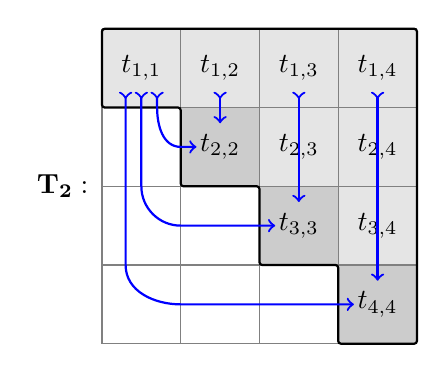
\begin{tikzpicture}[scale=1,every node/.style={minimum size=0.5cm}]

  \begin{scope}
    \fill[white,fill opacity=0.8] (0.0,0.0) rectangle (4.0,4.0);

    \fill[gray!20] (0,4) -- (0,3) -- (1,3) -- (1,2) -- (2,2) -- (2,1) -- (3,1) -- (3,0) -- (4,0) -- (4,4) -- cycle;

    \fill[gray!40] (1,3) -- (2,3) -- (2,2) -- (3,2) -- (3,1) -- (4,1) -- (4,0)
    -- (3,0) -- (3,1) -- (2,1) -- (2,2) -- (1,2) -- cycle;

    \draw[step=10mm, thin, gray] (0.0,0.0) grid (4.0,4.0);
    \draw[black, thick, rounded corners=1] (0,4) -- (0,3) -- (1,3) -- (1,2) -- (2,2) -- (2,1) -- (3,1) -- (3,0) -- (4,0) -- (4,4) -- cycle;

    \node at (0.5, 3.5) [black] {$t_{1,1}$};
    \node at (1.5, 3.5) [black] {$t_{1,2}$};
    \node at (2.5, 3.5) [black] {$t_{1,3}$};
    \node at (3.5, 3.5) [black] {$t_{1,4}$};
    \node at (1.5, 2.5) [black] {$t_{2,2}$};
    \node at (2.5, 2.5) [black] {$t_{2,3}$};
    \node at (3.5, 2.5) [black] {$t_{2,4}$};
    \node at (2.5, 1.5) [black] {$t_{3,3}$};
    \node at (3.5, 1.5) [black] {$t_{3,4}$};
    \node at (3.5, 0.5) [black] {$t_{4,4}$};

    \draw[>->, blue, thick] (0.7, 3.2) -- (0.7, 3) to[out=270,in=180] (1, 2.5) -- (1.2, 2.5);
    \draw[>->, blue, thick] (1.5, 3.2) -- (1.5, 2.8);
    \draw[>->, blue, thick] (0.5, 3.2) -- (0.5, 2) to[out=270,in=180] (1, 1.5) -- (2.2, 1.5);
    \draw[>->, blue, thick] (2.5, 3.2) -- (2.5, 1.8);
    \draw[>->, blue, thick] (0.3, 3.2) -- (0.3, 1) to[out=270,in=180] (1, 0.5) -- (3.2, 0.5);
    \draw[>->, blue, thick] (3.5, 3.2) -- (3.5, 0.8);
  \end{scope}

  \node at (-0.5, 2) [black] {$\mathbf{T_2}:$};
\end{tikzpicture}
\end{document}

  }
  \qquad
  \subfloat[][]{
    \documentclass{standalone}
\usepackage{tikz}

\begin{document}
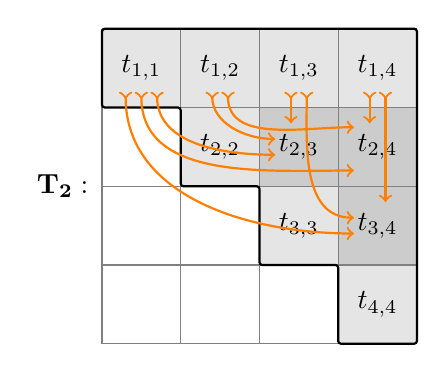
\begin{tikzpicture}[scale=1,every node/.style={minimum size=0.5cm}]

  \begin{scope}
    \fill[white,fill opacity=0.8] (0.0,0.0) rectangle (4.0,4.0);

    \fill[gray!20] (0,4) -- (0,3) -- (1,3) -- (1,2) -- (2,2) -- (2,1) -- (3,1) -- (3,0) -- (4,0) -- (4,4) -- cycle;

    \fill[gray!40] (2,3) -- (4,3) -- (4,1) -- (3,1) -- (3,2) -- (2,2) -- cycle;

    \draw[step=10mm, thin, gray] (0.0,0.0) grid (4.0,4.0);
    \draw[black, thick, rounded corners=1] (0,4) -- (0,3) -- (1,3) -- (1,2) -- (2,2) -- (2,1) -- (3,1) -- (3,0) -- (4,0) -- (4,4) -- cycle;

    \node at (0.5, 3.5) [black] {$t_{1,1}$};
    \node at (1.5, 3.5) [black] {$t_{1,2}$};
    \node at (2.5, 3.5) [black] {$t_{1,3}$};
    \node at (3.5, 3.5) [black] {$t_{1,4}$};
    \node at (1.5, 2.5) [black] {$t_{2,2}$};
    \node at (2.5, 2.5) [black] {$t_{2,3}$};
    \node at (3.5, 2.5) [black] {$t_{2,4}$};
    \node at (2.5, 1.5) [black] {$t_{3,3}$};
    \node at (3.5, 1.5) [black] {$t_{3,4}$};
    \node at (3.5, 0.5) [black] {$t_{4,4}$};

    \draw[>->, orange, thick] (1.4, 3.2) to[out=270,in=180] (2.2, 2.6);
    \draw[>->, orange, thick] (2.4, 3.2) to[out=270,in=90] (2.4, 2.8);
    \draw[>->, orange, thick] (0.7, 3.2) to[out=270,in=180] (2.2, 2.4);

    \draw[>->, orange, thick] (1.6, 3.2) to[out=270,in=180] (3.2, 2.75);
    \draw[>->, orange, thick] (3.4, 3.2) to[out=270,in=90] (3.4, 2.8);
    \draw[>->, orange, thick] (0.5, 3.2) to[out=270,in=180] (3.2, 2.2);


    \draw[>->, orange, thick] (2.6, 3.2) to[out=270,in=180] (3.2, 1.6);
    \draw[>->, orange, thick] (3.6, 3.2) to[out=270,in=90] (3.6, 1.8);
    \draw[>->, orange, thick] (0.3, 3.2) to[out=270,in=180] (3.2, 1.4);

  \end{scope}

  \node at (-0.5, 2) [black] {$\mathbf{T_2}:$};
\end{tikzpicture}
\end{document}

  }
\caption{Oscillator matrix update going from $\mat{T_1}$ to $\mat{T_2}$}
\label{fig:oscillator_update_T1}
\end{figure}

\begin{figure}
  \centering
  \subfloat[][]{
    \documentclass{standalone}
\usepackage{tikz}

\begin{document}
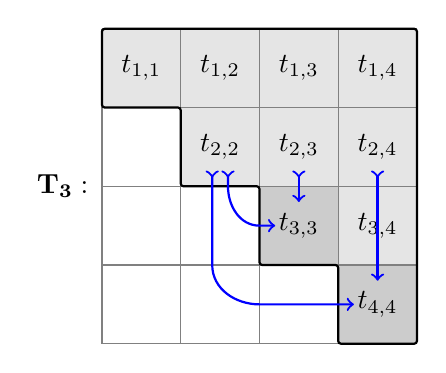
\begin{tikzpicture}[scale=1,every node/.style={minimum size=0.5cm}]

  \begin{scope}
    \fill[white,fill opacity=0.8] (0.0,0.0) rectangle (4.0,4.0);

    \fill[gray!20] (0,4) -- (0,3) -- (1,3) -- (1,2) -- (2,2) -- (2,1) -- (3,1) -- (3,0) -- (4,0) -- (4,4) -- cycle;

    \fill[gray!40] (2,2) -- (3,2) -- (3,1) -- (4,1) -- (4,0) -- (3,0) -- (3,1)
    -- (2,1) --cycle;

    \draw[step=10mm, thin, gray] (0.0,0.0) grid (4.0,4.0);
    \draw[black, thick, rounded corners=1] (0,4) -- (0,3) -- (1,3) -- (1,2) -- (2,2) -- (2,1) -- (3,1) -- (3,0) -- (4,0) -- (4,4) -- cycle;

    \node at (0.5, 3.5) [black] {$t_{1,1}$};
    \node at (1.5, 3.5) [black] {$t_{1,2}$};
    \node at (2.5, 3.5) [black] {$t_{1,3}$};
    \node at (3.5, 3.5) [black] {$t_{1,4}$};
    \node at (1.5, 2.5) [black] {$t_{2,2}$};
    \node at (2.5, 2.5) [black] {$t_{2,3}$};
    \node at (3.5, 2.5) [black] {$t_{2,4}$};
    \node at (2.5, 1.5) [black] {$t_{3,3}$};
    \node at (3.5, 1.5) [black] {$t_{3,4}$};
    \node at (3.5, 0.5) [black] {$t_{4,4}$};

    \draw[>->, blue, thick] (1.6, 2.2) -- (1.6, 2) to[out=270,in=180] (2, 1.5) -- (2.2, 1.5);
    \draw[>->, blue, thick] (2.5, 2.2) -- (2.5, 1.8);
    \draw[>->, blue, thick] (1.4, 2.2) -- (1.4, 1) to[out=270,in=180] (2, 0.5) -- (3.2, 0.5);
    \draw[>->, blue, thick] (3.5, 2.2) -- (3.5, 0.8);
  \end{scope}

  \node at (-0.5, 2) [black] {$\mathbf{T_3}:$};
\end{tikzpicture}
\end{document}

  }
  \qquad
  \subfloat[][]{
    \documentclass{standalone}
\usepackage{tikz}

\begin{document}
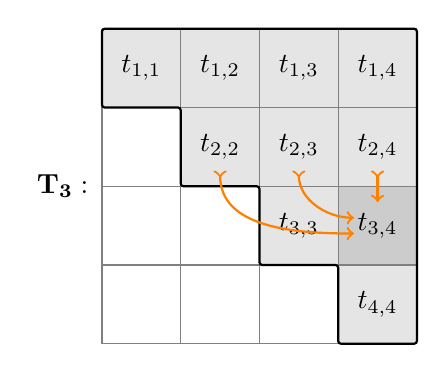
\begin{tikzpicture}[scale=1,every node/.style={minimum size=0.5cm}]

  \begin{scope}
    \fill[white,fill opacity=0.8] (0.0,0.0) rectangle (4.0,4.0);

    \fill[gray!20] (0,4) -- (0,3) -- (1,3) -- (1,2) -- (2,2) -- (2,1) -- (3,1) -- (3,0) -- (4,0) -- (4,4) -- cycle;

    \fill[gray!40] (3,2) -- (4,2) -- (4,1) -- (3,1) -- cycle;

    \draw[step=10mm, thin, gray] (0.0,0.0) grid (4.0,4.0);
    \draw[black, thick, rounded corners=1] (0,4) -- (0,3) -- (1,3) -- (1,2) -- (2,2) -- (2,1) -- (3,1) -- (3,0) -- (4,0) -- (4,4) -- cycle;

    \node at (0.5, 3.5) [black] {$t_{1,1}$};
    \node at (1.5, 3.5) [black] {$t_{1,2}$};
    \node at (2.5, 3.5) [black] {$t_{1,3}$};
    \node at (3.5, 3.5) [black] {$t_{1,4}$};
    \node at (1.5, 2.5) [black] {$t_{2,2}$};
    \node at (2.5, 2.5) [black] {$t_{2,3}$};
    \node at (3.5, 2.5) [black] {$t_{2,4}$};
    \node at (2.5, 1.5) [black] {$t_{3,3}$};
    \node at (3.5, 1.5) [black] {$t_{3,4}$};
    \node at (3.5, 0.5) [black] {$t_{4,4}$};

    \draw[>->, orange, thick] (2.5, 2.2) to[out=270,in=180] (3.2, 1.6);
    \draw[>->, orange, thick] (3.5, 2.2) to[out=270,in=90] (3.5, 1.8);
    \draw[>->, orange, thick] (1.5, 2.2) to[out=270,in=180] (3.2, 1.4);
  \end{scope}

  \node at (-0.5, 2) [black] {$\mathbf{T_3}:$};
\end{tikzpicture}
\end{document}
  }
\caption{Oscillator matrix update going from $\mat{T_2}$ to $\mat{T_3}$}
\label{fig:oscillator_update_T2}
\end{figure}

\begin{figure}
  \centering
  \subfloat[][]{
    \documentclass{standalone}
\usepackage{tikz}

\begin{document}
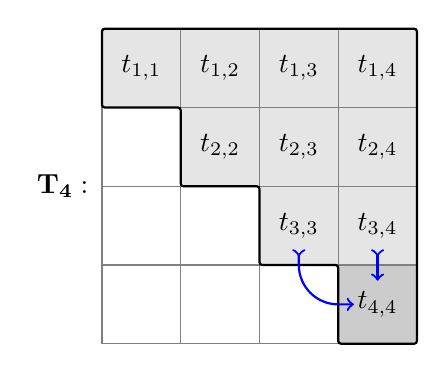
\begin{tikzpicture}[scale=1,every node/.style={minimum size=0.5cm}]

  \begin{scope}
    \fill[white,fill opacity=0.8] (0.0,0.0) rectangle (4.0,4.0);

    \fill[gray!20] (0,4) -- (0,3) -- (1,3) -- (1,2) -- (2,2) -- (2,1) -- (3,1) -- (3,0) -- (4,0) -- (4,4) -- cycle;

    \fill[gray!40] (3,1) -- (4,1) -- (4,0) -- (3,0) -- cycle;

    \draw[step=10mm, thin, gray] (0.0,0.0) grid (4.0,4.0);
    \draw[black, thick, rounded corners=1] (0,4) -- (0,3) -- (1,3) -- (1,2) -- (2,2) -- (2,1) -- (3,1) -- (3,0) -- (4,0) -- (4,4) -- cycle;

    \node at (0.5, 3.5) [black] {$t_{1,1}$};
    \node at (1.5, 3.5) [black] {$t_{1,2}$};
    \node at (2.5, 3.5) [black] {$t_{1,3}$};
    \node at (3.5, 3.5) [black] {$t_{1,4}$};
    \node at (1.5, 2.5) [black] {$t_{2,2}$};
    \node at (2.5, 2.5) [black] {$t_{2,3}$};
    \node at (3.5, 2.5) [black] {$t_{2,4}$};
    \node at (2.5, 1.5) [black] {$t_{3,3}$};
    \node at (3.5, 1.5) [black] {$t_{3,4}$};
    \node at (3.5, 0.5) [black] {$t_{4,4}$};

    \draw[>->, blue, thick] (2.5, 1.2) -- (2.5, 1) to[out=270,in=180] (3, 0.5) -- (3.2, 0.5);
    \draw[>->, blue, thick] (3.5, 1.2) -- (3.5, 0.8);

  \end{scope}

  \node at (-0.5, 2) [black] {$\mathbf{T_4}:$};
\end{tikzpicture}
\end{document}

  }
  \qquad
  \subfloat[][]{
    \documentclass{standalone}
\usepackage{tikz}

\begin{document}
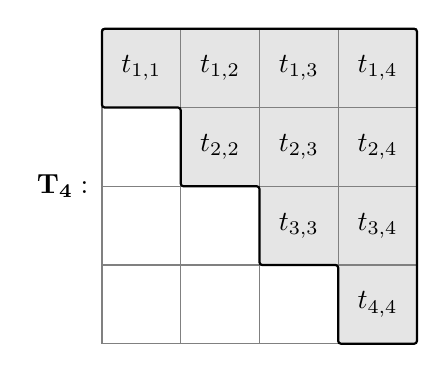
\begin{tikzpicture}[scale=1,every node/.style={minimum size=0.5cm}]

  \begin{scope}
    \fill[white,fill opacity=0.8] (0.0,0.0) rectangle (4.0,4.0);

    \fill[gray!20] (0,4) -- (0,3) -- (1,3) -- (1,2) -- (2,2) -- (2,1) -- (3,1) -- (3,0) -- (4,0) -- (4,4) -- cycle;
    \draw[step=10mm, thin, gray] (0.0,0.0) grid (4.0,4.0);
    \draw[black, thick, rounded corners=1] (0,4) -- (0,3) -- (1,3) -- (1,2) -- (2,2) -- (2,1) -- (3,1) -- (3,0) -- (4,0) -- (4,4) -- cycle;

    \node at (0.5, 3.5) [black] {$t_{1,1}$};
    \node at (1.5, 3.5) [black] {$t_{1,2}$};
    \node at (2.5, 3.5) [black] {$t_{1,3}$};
    \node at (3.5, 3.5) [black] {$t_{1,4}$};
    \node at (1.5, 2.5) [black] {$t_{2,2}$};
    \node at (2.5, 2.5) [black] {$t_{2,3}$};
    \node at (3.5, 2.5) [black] {$t_{2,4}$};
    \node at (2.5, 1.5) [black] {$t_{3,3}$};
    \node at (3.5, 1.5) [black] {$t_{3,4}$};
    \node at (3.5, 0.5) [black] {$t_{4,4}$};
  \end{scope}

  \node at (-0.5, 2) [black] {$\mathbf{T_4}:$};
\end{tikzpicture}
\end{document}
  }
\caption{Oscillator matrix update going from $\mat{T_3}$ to $\mat{T_4}$}
\label{fig:oscillator_update_T3}
\end{figure}


\subsection{Semi-open issue: Solving the path equations}

The topic of this section is the path equation for $g_i$ and how to
solve it. We will use formula \eqref{eq:general_partial_g} in combination
with \eqref{eq:stationary_point} and \eqref{eq:general_ki}. The path equation
for $g_i$ reads:

\begin{equation*}
  g_i\left(h_i\left(\tau_i, x_{i+1}, \ldots, x_N\right), x_{i+1}, \ldots, x_N\right)
  = g_i\left(x_i^{*}\left(x_{i+1}, \ldots, x_N\right), x_{i+1}, \ldots, x_N\right) + i \tau_i
\end{equation*}

where we neglect in the notation the dependence of $g_i$, $h_i$ and $x_i^{**}$ on $x_j$
for $j>i$ and simply write:

\begin{equation} \label{eq:general_path_eqn}
  g_i\left(h_i\left(\tau_i\right)\right) = g_i\left(x_i^{**}\right) + i \tau_i \,.
\end{equation}

Expanding the left side:

\begin{equation}
\begin{split}
  g_i\left(h_i\right)
  & = t_{i,i} h_i^2 + \sum_{j=i+1}^{N} t_{i,j} h_i x_j
    = t_{i,i} h_i^2 +  h_i \sum_{j=i+1}^{N} t_{i,j} x_j
\end{split}
\end{equation}

and combine both sides:

\begin{equation}
  \underbrace{t_{i,i}}_{A} h_i^2
  +
  h_i \underbrace{\sum_{j=i+1}^{N} t_{i,j} x_j}_{B}
  +
  \underbrace{\frac{1}{4 t_{i,i}} \left( \sum_{j=i+1}^{N} t_{i,j} x_j \right)^2 - i \tau_i}_{C}
  = 0
\end{equation}

we get a simple quadratic equation for $h_i$. Its solution
is given by:

\begin{equation}
  h_i = \frac{-B \pm \sqrt{\Delta}}{2 A}
  \quad \text{where} \quad
  \Delta \assign B^2 - 4 A C \,.
\end{equation}

The discriminant seems to be complicated at the first sight:

\begin{equation}
\begin{split}
  \Delta & = B^2 - 4 A C
  = \left(\sum_{j=i+1}^{N} t_{i,j} x_j\right)^2
    - 4 t_{i,i} \left(\frac{1}{4 t_{i,i}} \left( \sum_{j=i+1}^{N} t_{i,j} x_j \right)^2 - i \tau_i\right) \\
  & = \left(\sum_{j=i+1}^{N} t_{i,j} x_j\right)^2
      - 4 t_{i,i} \frac{1}{4 t_{i,i}} \left( \sum_{j=i+1}^{N} t_{i,j} x_j \right)^2
      + 4 t_{i,i} i \tau_i \\
  & = 4 t_{i,i} i \tau_i
\end{split}
\end{equation}

but actually is surprisingly simple. For the complete path we
then get:

\begin{equation}
  h_i = \frac{-\sum_{j=i+1}^{N} t_{i,j} x_j \pm \sqrt{4 t_{i,i} i \tau_i}}
             {2 t_{i,i}}
\end{equation}

which transforms into a nicer version:

\begin{equation} \label{eq:general_path_formula}
\boxed{
  h_i\left(\tau_i, x_{i+1}, \ldots, x_N\right)
  = -\frac{1}{2 t_{i,i}} \sum_{j=i+1}^{N} t_{i,j} x_j \pm \sqrt{\frac{i \tau_i}{t_{i,i}}}
}
\end{equation}

where we retrieve the decoupled formula from the symmetric case
as soon as $t_{i,j} = 0$ for all $i \neq j$. It is important to note
that the whole path depends only \emph{linearly} on the remaining
higher variables $x_j$ with $j>i$.

In a next step we can easily compute the derivative of any
path:

\begin{equation}
\begin{split}
  \pdiff{h_i}{\tau_i}
  & = \pdiff{}{\tau_i}
      \left(-\frac{1}{2 t_{i,i}} \sum_{j=i+1}^{N} t_{i,j} x_j \pm \sqrt{\frac{i \tau_i}{t_{i,i}}}\right) \\
  & = \pm \pdiff{}{\tau_i} \sqrt{\frac{i \tau_i}{t_{i,i}}}
\end{split}
\end{equation}

and find this simple expression:

\begin{equation} \label{eq:general_path_derivative_formula}
\boxed{
  h_i^{\prime} \assign \pdiff{h_i\left(\tau_i\right)}{\tau_i}
  = \pm \frac{(-1)^{\frac{1}{4}}}{2 \sqrt{t_{i,i}}\sqrt{\tau_i}} \,.
}
\end{equation}

Formula \eqref{eq:general_path_formula} allows us to compute explicitly
starting with $h_N$ all paths $h_{N-1}, h_{N-2}, \ldots$ up to $h_1$
in this reversed order. It is obvious that for these formulae to be valid
$t_{i,i}$ must never be zero.


\subsection{Semi-open issue: general case with shift}

This time we try to solve the full problem:

\begin{equation}
  g\left(\vec{x}\right) \assign \vec{x}\T \mat{A} \vec{x} + \vec{b}\T \vec{x} + c
\end{equation}

\marginpar{Do this for complex $\mat{A}$.}

where we do not make any assumptions on $\mat{A}$ beside of being real and invertible.
First we complete the square. Starting from the above oscillator we want to find
a transformation to get rid of the linear term. Assuming that the transformation
is linear:

\begin{equation}
 \vec{\tilde{x}} = \chi^{-1}\left(\vec{x}\right) := \vec{x} - \vec{u}
 \quad \leftrightarrow \quad
 \vec{x} = \chi\left(\vec{\tilde{x}}\right) = \vec{\tilde{x}} + \vec{u} \,.
\end{equation}

we find that:

\begin{equation}
\begin{split}
  \vec{\tilde{x}}\T \mat{A} \vec{\tilde{x}}
  & = \left(\vec{x}-\vec{u}\right)\T \mat{A} \left(\vec{x}-\vec{u}\right) \\
  & = \vec{x}\T \mat{A} \vec{x} - \vec{x}\T \mat{A} \vec{u} -
      \vec{u}\T \mat{A} \vec{x} + \vec{u}\T \mat{A} \vec{u} \\
  & = \vec{x}\T \mat{A} \vec{x} - \vec{u}\T \mat{A}\T \vec{x} -
      \vec{u}\T \mat{A} \vec{x} + \vec{u}\T \mat{A} \vec{u} \,.
\end{split}
\end{equation}

If we match this against the definition of $g$ we get the
relations shown next. We are interested in the linear terms
for finding $\vec{u}$:

\begin{equation}
\begin{split}
  \vec{b}\T \vec{x} & = - \vec{u}\T \mat{A}\T \vec{x} - \vec{u}\T \mat{A} \vec{x} \\
  \vec{b}\T         & = - \vec{u}\T \left(\mat{A} + \mat{A}\T\right) \\
  \vec{b}           & = - \left(\mat{A} + \mat{A}\T\right) \vec{u} \\
\end{split}
\end{equation}

and finally:

\begin{equation}
  \vec{u} = - \left(\mat{A} + \mat{A}\T\right)\inv \vec{b} \,.
\end{equation}

With the explicit value of $u$ we can rewrite our $\chi$ in a final form:

\begin{equation}
 \vec{\tilde{x}} = \chi^{-1}\left(\vec{x}\right) := \vec{x} + \left(\mat{A} + \mat{A}\T\right)\inv \vec{b}
 \quad \leftrightarrow \quad
 \vec{x} = \chi\left(\vec{\tilde{x}}\right) = \vec{\tilde{x}} - \left(\mat{A} + \mat{A}\T\right)\inv \vec{b} \,.
\end{equation}

Then we can start computing the new oscillator $\tilde{g}$:

\begin{equation}
\begin{split}
  g\left(\vec{x}\right)
  & =g\left(\chi\left(\vec{\tilde{x}}\right)\right) \\
  & = \left(\vec{\tilde{x}} - \left(\mat{A} + \mat{A}\T\right)\inv \vec{b}\right)\T
      \mat{A}
      \left(\vec{\tilde{x}} - \left(\mat{A} + \mat{A}\T\right)\inv \vec{b}\right)
      + \vec{b}\T \left(\vec{\tilde{x}} - \left(\mat{A} + \mat{A}\T\right)\inv \vec{b}\right)
      + c \\
% \end{split}
% \end{equation}
\intertext{we expand and simplify this step by step:}
% \begin{equation}
% \begin{split}
  & =   \vec{\tilde{x}}\T \mat{A} \vec{\tilde{x}}
      - \vec{\tilde{x}}\T \mat{A} \left(\mat{A} + \mat{A}\T\right)\inv \vec{b}
      - \left(\left(\mat{A} + \mat{A}\T\right)\inv \vec{b}\right)\T \mat{A} \vec{\tilde{x}} \\
  & \quad
      + \left(\left(\mat{A} + \mat{A}\T\right)\inv \vec{b}\right)\T \mat{A} \left(\mat{A} + \mat{A}\T\right)\inv \vec{b}
      + \vec{b}\T \left(\vec{\tilde{x}} - \left(\mat{A} + \mat{A}\T\right)\inv \vec{b}\right)
      + c \\
  & =   \vec{\tilde{x}}\T \mat{A} \vec{\tilde{x}}
      - \vec{\tilde{x}}\T \mat{A} \left(\mat{A} + \mat{A}\T\right)\inv \vec{b}
      - \vec{b}\T \left(\mat{A} + \mat{A}\T\right)\Tinv \mat{A} \vec{\tilde{x}} \\
  & \quad
      + \vec{b}\T \left(\mat{A} + \mat{A}\T\right)\Tinv \mat{A} \left(\mat{A} + \mat{A}\T\right)\inv \vec{b}
      + \vec{b}\T \vec{\tilde{x}} - \vec{b}\T \left(\mat{A} + \mat{A}\T\right)\inv \vec{b}
      + c \,.
\end{split}
\end{equation}

In a next step, try to unify the linear terms having only one $\vec{\tilde{x}}$:

\begin{equation}
\begin{split}
   &- \vec{\tilde{x}}\T \mat{A} \left(\mat{A} + \mat{A}\T\right)\inv \vec{b}
    - \vec{b}\T \left(\mat{A} + \mat{A}\T\right)\Tinv \mat{A} \vec{\tilde{x}}
    + \vec{b}\T \vec{\tilde{x}} \\
 = &- \vec{b}\T \left(\mat{A} + \mat{A}\T\right)\Tinv \mat{A}\T \vec{\tilde{x}}
    - \vec{b}\T \left(\mat{A} + \mat{A}\T\right)\Tinv \mat{A} \vec{\tilde{x}}
    + \vec{b}\T \vec{\tilde{x}} \\
 = &- \vec{b}\T
      \left(
        \left(\mat{A} + \mat{A}\T\right)\inv \mat{A}\T
      + \left(\mat{A} + \mat{A}\T\right)\inv \mat{A}
      \right)
      \vec{\tilde{x}}
    + \vec{b}\T \vec{\tilde{x}} \\
 = &- \vec{b}\T
      \left(\mat{A} + \mat{A}\T\right)\inv
      \left(\mat{A} + \mat{A}\T\right)
      \vec{\tilde{x}}
    + \vec{b}\T \vec{\tilde{x}} \\
 = &- \vec{b}\T \vec{\tilde{x}}
    + \vec{b}\T \vec{\tilde{x}} = 0 \,.
\end{split}
\end{equation}

and indeed we find that they vanish. This confirmes that the
transformation is correct. At the end of the day we obtain the
new oscillator free of any linear term:

\begin{equation}
  \tilde{g}\left(\vec{\tilde{x}}\right) \assign
  \vec{\tilde{x}}\T \mat{A} \vec{\tilde{x}}
  + \vec{b}\T \left(\mat{A} + \mat{A}\T\right)\Tinv \mat{A} \left(\mat{A} + \mat{A}\T\right)\inv \vec{b}
  - \vec{b}\T \left(\mat{A} + \mat{A}\T\right)\inv \vec{b}
  + c
\end{equation}

where we can pack all the constant terms into the definition of $\tilde{c}$:

\begin{equation}
\begin{split}
  \tilde{c} & \assign
              \vec{b}\T \left(\mat{A} + \mat{A}\T\right)\Tinv \mat{A} \left(\mat{A} + \mat{A}\T\right)\inv \vec{b}
            - \vec{b}\T \left(\mat{A} + \mat{A}\T\right)\inv \vec{b}
            + c \\
            & =
            -\frac{1}{2} \vec{b}\T \left(\mat{A} + \mat{A}\T\right)\inv \vec{b} + c \,.
\end{split}
\end{equation}

Therefore:

\begin{equation}
  \tilde{g}\left(\vec{\tilde{x}}\right) = \vec{\tilde{x}}\T \mat{A} \vec{\tilde{x}}
                                        -\frac{1}{2} \vec{b}\T \left(\mat{A} + \mat{A}\T\right)\inv \vec{b} + c
\end{equation}


\subsection{Semi-open issue: performing the Schur decomposition}


Given an oscillator with a general matrix $\mat{A}$ as:

\begin{equation}
  g\left(\vec{x}\right) \assign \vec{x}\T \mat{A} \vec{x} + c \,.
\end{equation}

We seek a coordinate transformation that makes the matrix $\mat{A}$
(upper) triagonal. This is achieved by the Schur decomposition:

\begin{equation}
 \mat{A} = \mat{U}\H \mat{T} \mat{U}
\end{equation}

where $\mat{U}$ is even unitary. The transformation is then given
by the following mapping:

\begin{equation}
 \vec{\hat{x}} = \rho^{-1}\left(\vec{x}\right) := \mat{U} \vec{x}
 \quad \leftrightarrow \quad
 \vec{x} = \rho\left(\vec{\hat{x}}\right) = \mat{U}\inv \vec{\hat{x}} = \mat{U}\T \vec{\hat{x}} \,.
\end{equation}

For the oscillator we compute:

\begin{equation}
\begin{split}
 g\left(\vec{x}\right) & = g\left(\rho\left(\vec{\hat{x}}\right)\right)
                         = g\left(\mat{U}\T \vec{\hat{x}}\right) \\
 & = \left(\mat{U}\T \vec{\hat{x}}\right)\T \mat{A} \left(\mat{U}\T \vec{\hat{x}}\right)
   + c \\
 & = \vec{\hat{x}}\T \mat{U} \mat{A} \mat{U}\T \vec{\hat{x}}
   + c \\
 & = \vec{\hat{x}}\T \mat{T} \vec{\hat{x}}
   + c
\end{split}
\end{equation}

with $\mat{T}$ upper triagonal. Finally we have:

\begin{equation}
  \hat{g}\left(\vec{\hat{x}}\right) \assign \vec{\hat{x}}\T \mat{T} \vec{\hat{x}} + c \,.
\end{equation}

Therefore we have:

\begin{equation}
  \hat{g}\left(\vec{\hat{x}}\right) = g\left(\chi\left(\rho\left(\vec{\hat{x}}\right)\right)\right)
                                    = g\left(\tau\left(\vec{\hat{x}}\right)\right)
\end{equation}

and we can reduce any quadratic oscillator to a triagonal normal form.
The related transformation $\tau$ is a composition of $\chi$ and $\rho$:

\begin{equation}
\begin{split}
  \vec{\hat{x}} & = \tau\inv \left(\vec{x}\right)
                  = \rho\inv \left( \chi\inv \left(\vec{x}\right) \right)
                  = \rho\inv \left(\vec{x} + \left(\mat{A} + \mat{A}\T\right)\inv \vec{b}\right)
                  = \mat{U} \vec{x} + \mat{U} \left(\mat{A} + \mat{A}\T\right)\inv \vec{b} \\
  \vec{x} & = \tau \left(\vec{\hat{x}}\right)
            = \chi \left( \rho \left(\vec{\hat{x}}\right) \right)
            = \chi \left( \mat{U}\T \vec{\hat{x}} \right)
            = \mat{U}\T \vec{\hat{x}} - \left(\mat{A} + \mat{A}\T\right)\inv \vec{b}
\end{split}
\end{equation}



\section{On wavepackets and oscillators}

In this section we look at the wavepackets involved in the computation
of overlap integrals. Each wavepacket $\phi$ is of the form:

\begin{equation}
  \phi(\vec{x}) \sim p(x)\exp\left(\frac{i}{\varepsilon^2} g(x)\right) \,.
\end{equation}

This is sufficient for the steepest descent technique to be applicable.
Indeed, comparing to the integrand in \eqref{eq:oscillatory_integral},
we find that $\omega = \frac{1}{\varepsilon^2}$. The method becomes
better the smaller $\varepsilon$ is.

The actual oscillator $g$ is of the form:

\begin{equation}
  g\left(\vec{x}\right)
  \assign
  \frac{1}{2} \dotp{\vec{x}-\vec{q}}{\mat{P}\mat{Q}\inv \left(\vec{x}-\vec{q}\right)}
  +
  \dotp{\vec{p}}{\vec{x}-\vec{q}}
\end{equation}

Usually we are interested in integrals of the form $\dotp{\phi_k}{\phi_l}$.
In that case the integral is still of the same oscillatory structure:

\begin{equation}
\begin{split}
  \dotp{\phi_k}{\phi_l} & =
  \int_{-\infty}^{\infty} \conj{p_k(x)\exp\left(\frac{i}{\varepsilon^2} g_k(x)\right)}
                                p_l(x)\exp\left(\frac{i}{\varepsilon^2} g_l(x)\right)
  \mathrm{d}\vec{x} \\
  & =
  \int_{-\infty}^{\infty}
    \conj{p_k(x)} p_l(x)
    \exp\left(-\frac{i}{\varepsilon^2} \conj{g_k(x)} + \frac{i}{\varepsilon^2} g_l(x)\right)
  \mathrm{d}\vec{x} \\
  & =
  \int_{-\infty}^{\infty}
    \conj{p_k(x)} p_l(x)
    \exp\left(\frac{i}{\varepsilon^2}\left(-\conj{g_k(x)} + g_l(x)\right)\right)
  \mathrm{d}\vec{x} \,.
\end{split}
\end{equation}

The next step to take is to combine both oscillators $g_k$ and $g_l$ into a
single one such that we get back a formal expression like the one in
\eqref{eq:oscillatory_integral} we started with.

\subsection{Combining different oscillators}

Combining the two oscillators is actually a straight-forward computation,
however it is very error prone, big chances are that we miss a transpose
or conjugate somewhere. To simplify the notation define:

\begin{equation}
  \mat{\Gamma_i} \assign \mat{P_i}\mat{Q_i}\inv
\end{equation}

and start with computing $\conj{g_k}$:

\begin{equation}
\begin{split}
 \conj{g_k}
 & =
 \frac{1}{2}\conj{\dotp{\vec{x}-\vec{q_k}}{\mat{\Gamma_k} \left(\vec{x}-\vec{q_k}\right)}}
 +\conj{\dotp{\vec{p_k}}{\vec{x}-\vec{q_k}}} \\
 & =
 \frac{1}{2} \left(
                \conj{\dotp{\vec{x}}{\mat{\Gamma_k} \vec{x}}}
               -\conj{\dotp{\vec{x}}{\mat{\Gamma_k} \vec{q_k}}}
               -\conj{\dotp{\vec{q_k}}{\mat{\Gamma_k} \vec{x}}}
               +\conj{\dotp{\vec{q_k}}{\mat{\Gamma_k} \vec{q_k}}}
              \right)
 + \conj{\dotp{\vec{p_k}}{\vec{x}}}
 - \conj{\dotp{\vec{p_k}}{\vec{q_k}}} \\
 & =
 \frac{1}{2} \left(
               \vec{x}\H \mat{\Gamma_k}\H \vec{x}
              -\vec{q_k}\H \mat{\Gamma_k}\H \vec{x}
              -\vec{x}\H \mat{\Gamma_k}\H \vec{q_k}
              +\vec{q_k}\H \mat{\Gamma_k}\H \vec{q_k}
              \right)
 + \vec{x}\H \vec{p_k} - \vec{q_k}\H \vec{p_k} \,.
\end{split}
\end{equation}

Next we add $g_l$ and simplify the following expression:

\begin{equation}
\begin{split}
 -\conj{g_k} + g_l
 = &
 -\frac{1}{2} \left(
               \vec{x}\H \mat{\Gamma_k}\H \vec{x}
              -\vec{q_k}\H \mat{\Gamma_k}\H \vec{x}
              -\vec{x}\H \mat{\Gamma_k}\H \vec{q_k}
              +\vec{q_k}\H \mat{\Gamma_k}\H \vec{q_k}
              \right)
 - \left(\vec{x}\H \vec{p_k} - \vec{q_k}\H \vec{p_k}\right) \\
 & +
  \frac{1}{2} \left(
                \vec{x}\H \mat{\Gamma_l} \vec{x}
               -\vec{x}\H \mat{\Gamma_l} \vec{q_l}
               -\vec{q_l}\H \mat{\Gamma_l} \vec{x}
               +\vec{q_l}\H \mat{\Gamma_l} \vec{q_l}
              \right)
 + \left(\vec{p_l}\H \vec{x} - \vec{p_l}\H \vec{q_l}\right) \\
 = &
 \frac{1}{2} \left(\vec{x}\H \mat{\Gamma_l} \vec{x} - \vec{x}\H \mat{\Gamma_k}\H \vec{x}\right)
 +
 \frac{1}{2} \left(
               \vec{q_k}\H \mat{\Gamma_k}\H \vec{x}
              +\vec{x}\H \mat{\Gamma_k}\H \vec{q_k}
              -\vec{x}\H \mat{\Gamma_l} \vec{q_l}
              -\vec{q_l}\H \mat{\Gamma_l} \vec{x}
             \right) \\
 & +
 \left(\vec{p_l}\H \vec{x} - \vec{x}\H \vec{p_k}\right)
 + \frac{1}{2} \left(
                 \vec{q_l}\H \mat{\Gamma_l} \vec{q_l}
                -\vec{q_k}\H \mat{\Gamma_k}\H \vec{q_k}
               \right)
 + \left(\vec{q_k}\H \vec{p_k} - \vec{p_l}\H \vec{q_l}\right) \\
 = &
 \frac{1}{2} \vec{x}\H \left(\mat{\Gamma_l} - \mat{\Gamma_k}\H\right) \vec{x}
 + \frac{1}{2} \left(
                 \vec{q_k}\H \mat{\Gamma_k}\H \vec{x}
                -\vec{q_l}\H \mat{\Gamma_l} \vec{x}
                +\vec{q_k}\T \conj{\mat{\Gamma_k}} \conj{\vec{x}}
                -\vec{q_l}\T \mat{\Gamma_l}\T \conj{\vec{x}}
               \right) \\
 & +
 \left(\vec{p_l}\H \vec{x} - \vec{p_k}\T \conj{\vec{x}}\right)
 + \frac{1}{2} \left(
                 \vec{q_l}\H \mat{\Gamma_l} \vec{q_l}
                -\vec{q_k}\H \mat{\Gamma_k}\H \vec{q_k}
               \right)
 + \left(\vec{q_k}\H \vec{p_k} - \vec{p_l}\H \vec{q_l}\right) \,.
\end{split}
\end{equation}

In the end we find an oscillator of the usual normal form
% $g(\vec{x}) = \vec{x}\H \mat{A} \vec{x} + \vec{b}\H \vec{x} + c$
$g(\vec{x}) = \vec{x}\H \mat{A} \vec{x} + \vec{b}\T \vec{x} + c$
where:

\begin{equation} \label{eq:combined_oscillators}
\begin{split}
  \mat{A} & = \frac{1}{2} \left(\mat{\Gamma_l} - \mat{\Gamma_k}\H \right) \\
%   \vec{b} & = \left(\frac{1}{2} \left(
%                                   \vec{q_k}\H \mat{\Gamma_k}\H
%                                  -\vec{q_l}\H \mat{\Gamma_l}
%                                  +\vec{q_k}\T \conj{\mat{\Gamma_k}}
%                                  -\vec{q_l}\T \mat{\Gamma_l}\T
%                                 \right)
%                 + \left(\vec{p_l}\H - \vec{p_k}\T\right)
%               \right)\H \\
%           & = \frac{1}{2} \left(
%                             \mat{\Gamma_k} \vec{q_k}
%                            -\mat{\Gamma_l}\H \vec{q_l}
%                            +\mat{\Gamma_k}\T \conj{\vec{q_k}}
%                            -\conj{\mat{\Gamma_l}} \conj{\vec{q_l}}
%                           \right)
%               + \left(\vec{p_l} - \conj{\vec{p_k}}\right) \\
  \vec{b} & = \left(\frac{1}{2} \left(
                                  \vec{q_k}\H \mat{\Gamma_k}\H
                                 -\vec{q_l}\H \mat{\Gamma_l}
                                 +\vec{q_k}\T \conj{\mat{\Gamma_k}}
                                 -\vec{q_l}\T \mat{\Gamma_l}\T
                                \right)
                + \left(\vec{p_l}\H - \vec{p_k}\T\right)
              \right)\T \\
          & = \frac{1}{2} \left(
                            \conj{\mat{\Gamma_k}} \conj{\vec{q_k}}
                           -\mat{\Gamma_l}\T \conj{\vec{q_l}}
                           +\mat{\Gamma_k}\H \vec{q_k}
                           -\mat{\Gamma_l} \vec{q_l}
                          \right)
              + \left(\conj{\vec{p_l}} - \vec{p_k}\right) \\
  c & = \frac{1}{2} \left(
                      \vec{q_l}\H \mat{\Gamma_l} \vec{q_l}
                     -\vec{q_k}\H \mat{\Gamma_k}\H \vec{q_k}
                    \right)
        + \left(\vec{q_k}\H \vec{p_k} - \vec{p_l}\H \vec{q_l}\right)
\end{split}
\end{equation}

\marginpar{Do we need to split $\vec{b}$ in parts for $\vec{x}$ and $\conj{\vec{x}}$?}

and we assumed that $\vec{x}$ is real. Be sure to pay attention to
the fact that here we have $\vec{b}\T$ only instead of $\vec{b}\H$.


\section{Modified quadrature rule}

The generalized Gauss-Laguerre quadrature rule approximates
integrands as follows:

\begin{equation}
  \int_0^\infty f(x) \exp(-x) x^\alpha \mathrm{d}x
  \approx
  \sum_{k=1}^N f\left(\gamma_k\right) w_k \,.
\end{equation}

In our setting we do not know $f$ separately but only
in combination with $\exp(-x)$. Therefore we want to
approximate the integral instead:

\begin{equation}
  \int_0^\infty g(x) x^\alpha \mathrm{d}x
  \approx
  \sum_{k=1}^N g\left(\gamma_k^\prime\right) w_k^\prime
\end{equation}

with possibly different nodes and weights. We try to factor out
one exponential from the weights such that we can formally put
it into the $f$ part. The original formula for $w_k$ is:

\begin{equation}
  \vec{w}_k \assign
  \frac{\Gamma(\alpha+n)}{n \Gamma(n)}
  \frac{1}{L^{\alpha}_{n-1}\bigl(\vec{\gamma}_k\bigr) L^{\alpha+1}_{n-1}\bigl(\vec{\gamma}_k\bigr)} \,.
\end{equation}

The way we follow to achieve this goal is a bit long and cumbersome
but in the end we will get more than we asked for.

There is a connection between the Laguerre and Hermite polynomials
for the cases $\alpha = \pm \frac{1}{2}$:

\begin{equation}
\begin{split}
  H_{2n}(x) & = (-1)^n 2^{2n} n! \, L_n^{\left(-\frac{1}{2}\right)}(x^2) \\
  H_{2n+1}(x) & = (-1)^n 2^{2n+1} n! \, x \, L_n^{\left(\frac{1}{2}\right)}(x^2) \\
\end{split}
\end{equation}

Luckily these are the only two cases we need to consider anyway.
From above by algebraic manipulation we find:

\begin{equation}
\begin{split}
  L_n^{\left(-\frac{1}{2}\right)}(x^2) & = \frac{1}{(-1)^n 2^{2n} n!} H_{2n}(x) \\
  L_n^{\left(\frac{1}{2}\right)}(x^2)  & = \frac{1}{(-1)^n 2^{2n+1} n!} \frac{1}{x} H_{2n+1}(x)
\end{split}
\end{equation}

The next step is to exploit a connection between Hermite
polynomials $H_n$ and Hermite functions $h_n$:

\begin{equation}
  h_n(x) \assign \frac{1}{\sqrt{2^n n! \sqrt{\pi}}}
                 \exp\left(-\frac{x^2}{2}\right)
                 H_n(x) \,.
\end{equation}

From that equation we get:

\begin{equation}
  H_n(x) = \sqrt{2^n n! \sqrt{\pi}} \frac{1}{\exp\left(-\frac{x^2}{2}\right)} h_n(x) \,.
\end{equation}

Plugging this into the above relations for $L_n^{\left(-\frac{1}{2}\right)}$ and $L_n^{\left(\frac{1}{2}\right)}$ we find:

\begin{equation}
\begin{split}
  L_n^{\left(-\frac{1}{2}\right)}(x) & = \frac{1}{(-1)^n 2^{2n} n!}
                                         \sqrt{2^{2n} (2n)! \sqrt{\pi}}
                                         \frac{1}{\exp\left(-\frac{x}{2}\right)}
                                         h_{2n}(\sqrt{x}) \\
  L_n^{\left(\frac{1}{2}\right)}(x) & = \frac{1}{(-1)^n 2^{2n+1} n!}
                                        \sqrt{2^{2n+1} (2n+1)! \sqrt{\pi}}
                                        \frac{1}{\exp\left(-\frac{x}{2}\right)}
                                        \frac{1}{\sqrt{x}}
                                        h_{2n+1}(\sqrt{x}) \,.
\end{split}
\end{equation}

Using these formulae to compute the quadrature weights we start with:

\begin{equation}
\begin{split}
  w_k =
  \frac{\Gamma(n-\frac{1}{2})}{n \Gamma(n)}
  \frac{
        (-1)^{n-1} 2^{2(n-1)} (n-1)!
        (-1)^{n-1} 2^{2(n-1)+1} (n-1)!
       }{
        \sqrt{2^{2(n-1)} (2(n-1))! \sqrt{\pi}}
        \sqrt{2^{2(n-1)+1} (2(n-1)+1)! \sqrt{\pi}}
        }
  \frac{
        \exp(-\frac{\gamma_k}{2}) \exp(-\frac{\gamma_k}{2}) \sqrt{\gamma_k}
       }{
        h_{2(n-1)}(\sqrt{\gamma_k})
        h_{2(n-1)+1}(\sqrt{\gamma_k})
       }
\end{split}
\end{equation}

Next we convert all factorials to gamma functions by applying the well known
relation that $k! = \Gamma(k+1)$:

\begin{equation}
\begin{split}
  w_k =
  \frac{\Gamma(n-\frac{1}{2})}{n \Gamma(n)}
  \frac{
        2^{2n-2} \Gamma(n)
        2^{2n-1} \Gamma(n)
       }{
        \sqrt{\pi}
        \sqrt{2^{2n-2}} \sqrt{\Gamma(2n-1)}
        \sqrt{2^{2n-1}} \sqrt{\Gamma(2n)}
        }
  \frac{
        \exp(-\gamma_k) \sqrt{\gamma_k}
       }{
        h_{2n-1}(\sqrt{\gamma_k})
        h_{2n-2}(\sqrt{\gamma_k})
       } \,.
\end{split}
\end{equation}

Now we can start expanding the gamma functions according to the
following set of identities:

\begin{equation}
\begin{split}
  \Gamma(k+1) & = k \Gamma(k) \\
  \Gamma(k-1) & = \frac{\Gamma(k)}{k-1} \\
  \Gamma(2k)  & = \frac{2^{2k-1}}{\sqrt{\pi}} \Gamma(k) \, \Gamma\left(n+\frac{1}{2}\right) \,.
\end{split}
\end{equation}

Doing this for the denominator term first and
then removing some square roots gives:

\begin{equation}
\begin{split}
  w_k =
  \frac{\Gamma(n+\frac{1}{2}-1)}{n \Gamma(n)}
  \frac{
        2^{4n-3}
        \Gamma(n) \Gamma(n)
        \sqrt{2n-1}
       }{
        \sqrt{\pi}
        \sqrt{2^{4n-3}}
        \Gamma(2n)
        }
  \frac{
        \exp(-\gamma_k) \sqrt{\gamma_k}
       }{
        h_{2n-1}(\sqrt{\gamma_k})
        h_{2n-2}(\sqrt{\gamma_k})
       } \,.
\end{split}
\end{equation}

and in turn using the second and third gamma identities we find:

\begin{equation}
\begin{split}
  w_k =
  \frac{\Gamma(n+\frac{1}{2})}{n \left(n-\frac{1}{2}\right) \Gamma(n)}
  \frac{
        2^{4n-3}
        \Gamma(n) \Gamma(n)
        \sqrt{2n-1}
        \sqrt{\pi}
       }{
        \sqrt{\pi}
        \sqrt{2^{4n-3}}
        2^{2n-1}
        \Gamma(n) \Gamma\left(n+\frac{1}{2}\right)
        }
  \frac{
        \exp(-\gamma_k) \sqrt{\gamma_k}
       }{
        h_{2n-1}(\sqrt{\gamma_k})
        h_{2n-2}(\sqrt{\gamma_k})
       }
\end{split}
\end{equation}

and after canceling out all gamma terms:

\begin{equation}
\begin{split}
  w_k & =
  \frac{1}{n \left(n-\frac{1}{2}\right)}
  \frac{
        2^{4n-3}
        \sqrt{2n-1}
       }{
        \sqrt{2^{8n-5}}
        }
  \frac{
        \exp(-\gamma_k) \sqrt{\gamma_k}
       }{
        h_{2n-1}(\sqrt{\gamma_k})
        h_{2n-2}(\sqrt{\gamma_k})
       } \\
  & =
  \frac{1}{n \left(n-\frac{1}{2}\right)}
  \frac{
        \sqrt{2n-1}
       }{
        \sqrt{2}
        }
  \frac{
        \exp(-\gamma_k) \sqrt{\gamma_k}
       }{
        h_{2n-1}(\sqrt{\gamma_k})
        h_{2n-2}(\sqrt{\gamma_k})
       } \,.
\end{split}
\end{equation}

Finally, we can write the weights $w_k$ in terms of Hermite functions as:

\begin{equation}
\boxed{
  w_k =
  \frac{
        \sqrt{2n-1}
       }{
        \sqrt{2}
        \left(n^2-\frac{n}{2}\right)}
  \frac{
        \exp(-\gamma_k) \sqrt{\gamma_k}
       }{
        h_{2n-2}(\sqrt{\gamma_k})
        h_{2n-1}(\sqrt{\gamma_k})
       } \,.
}
\end{equation}

What we gain is that we can evaluate exponentially decaying Hermite functions
instead of polynomials by a stable recursive scheme. On the other hand we pay
for this advantage by the factor 2 in the order. To compute nodes for a quadrature
of order $n$ we need to evaluate the two Hermite functions of order $2n-2$ and $2n-1$.


\section{Open issues}

Some open issues are:

\begin{itemize}
  \item We have to evaluate polynomials for higher order states $\phi_{k}$.
        This can destroy the whole nice convergence.
  \item We have to take care of the \emph{full} prefactors. This
        includes computing (fractional) powers of matrices. (The issue
        is solved now and the prefactors pose no new problems.)
  \item The number of paths grows exponentially with the dimension!
        Currently this makes the method not useful for $D$ larger than 3 or 4.
  \item It is not clear if we can encounter a degenerate oscillator and
        what the do in this case.
\end{itemize}


\bibliographystyle{plain}
\bibliography{nsd}

\end{document}
